\input{packages} 
\setlength{\parindent}{0 em}
\setlength{\parskip}{3ex plus 0.5ex minus 0.5ex}
\setlength{\textwidth}{6.5 in}
\setlength{\textheight}{8.5in}
\usepackage{xcolor}
\usepackage{graphicx}
\topmargin= -0.5in
\oddsidemargin= -0.10in
\newcommand\SI[2]{\em{#1}\sf{\ #2}}
\newcommand\ang[1]{#1$^{\circ}$}
\newcommand\num[1]{\em{#1}}
\newcommand\LS[1]{LS={#1}$^o$}
\newcommand\eg{{\em e.g.}}
\newcommand\heref[2]{\em{#1}\em{#2}}
\def\baselinestretch{1.7}
\newenvironment{singlespace} {\def\baselinestretch{1.}}


\begin{document}
\begin{singlespace}
\begin{frontmatter}
\title{Seasonal variations of Titan's upper atmosphere during the Cassini Mission}

\author[URCA]{Beno\^{i}t Seignovert\corref{correspondingauthor}}\ead{research@seignovert.fr}
\author[URCA]{Pascal Rannou}
\author[JPL]{Robert A. West}
\author[LESIA]{Sandrine Vinatier}

\address[URCA]{GSMA, Universit\'{e} de Reims Champagne-Ardenne, UMR 7331-GSMA, 51687 Reims, France}
\address[JPL]{Jet Propulsion Laboratory, California Institute of Technology, Pasadena, CA 91109, USA}
\address[LESIA]{LESIA-Observatoire de Paris, CNRS, UPMC, Universit\'{e} Paris-Diderot, 5 place Jules Janssen, 92195 Meudon, France}

\cortext[correspondingauthor]{Corresponding author}

\begin{abstract}
The 13 years of the Cassini mission provide a unique dataset monitoring the evolution of Titan's atmosphere between 
the middle of the northern winter up to the northern summer solstice.
\end{abstract}

\begin{keyword}
Cassini \sep Titan \sep Haze \sep Season cycle
\end{keyword}

\end{frontmatter}
\end{singlespace}


\begin{linenumbers}

%--------------------------------------------------------------------------------------|
\section{Introduction}

Titan is the only moon of the solar system with a thick hazy atmosphere which represents about 20\% of its apparent 
diameter. Its atmosphere is mainly composed of nitrogen and methane. The photo-dissociation of these molecules by the 
UV light in the upper part of the atmosphere leads to the production a large number other hydrocarbons and nitriles as 
trace species and to photochemical haze of aerosols. This haze is global and completely covers Titan. It controls 
the thermal balance through its visible and thermal infrared properties. It also veils the lower atmosphere and the 
surface that can be perceived in few methane windows in near infrared.

Although the haze was detected in the middle 70's, it was first imaged by Pionner 10 and the two Voyagers 
\citep{Smith1981, Smith1982, Sromovsky1981}. Titan's haze layer had several remarkable structures as a northern (winter) 
polarhood, an interhemispheric asymmetry and a thin global detached haze layer above the main global haze. It was 
readily though that the detached haze layer had a dynamical origin \citep{Smith1981}. Photometric analysis allowed 
to give the extinction properties of both hazes and to evaluated the effective radius of the aerosols in the detached 
haze ($\simeq$ 0.3 $\mu$m) and in the main haze ($\simeq$ 0.4 $\mu$m) \citep{Rages1983,Rages1983b}. Analysis show
that the detached haze layer appears due to a strong depletion in aerosols extinction around 300 km, yielding a distinct 
layer above the main haze with a maximum extinction located around {350} {km} \citep{Rages1983}. Its horizontal extent is 
very stable in pressure and it is reported at all the southern latitudes up to \ang{45}N where it connects to the northern 
polar hood. The detached haze layer could be seen again twenty years after the Voyager flybys \citep{Porco2005}. The 
main change was in its altitude at 515 km, that is 165 km higher than in 1981. Again, it was a fairly homogeneous global 
shell above the main haze at a constant altitude. The DHL was merging with the northern polarhood. Notably, while Voyager 
observations were performed after the northern spring equinox, Cassini early observations occured during the northern 
winter, that is half a season before the next northern spring equinox.
 
The first attempt to explain the observation of the DHL is proposed by \cite{Toon1992}. They used a 1D microphysical 
model where a {\em ad hoc} vertical wind is added to maintain aloft the particles at a constant altitude above the main 
haze. Alternative scenarii were proposed to explain the DHL from pure microphysical processes. \cite{Chassefiere1995} 
investigated the case of two different aerosol production layers. They proposed that the uppermost layer (500-1000 km) 
produces fluffy aggregates that could be swept horizontally by winds, generating a detached haze layer. They also 
propose an alternative scenario where aerosols settle downward and interact with macromolecules from the main haze, 
produced by the lower production zone (around 350-400 km). In the latter case, the interaction would produce by some 
way an optical gap. However, they clearly favorize the scenario involving winds which would match all the contraints 
known at that time. In the same vein, \cite{Lavvas2009} proposed a scenario based on a pure microphycal process. Aerosols 
are produced at high altitude (as in \cite{Chassefiere1995} hypothesis) growing as spheres down to levels around 500 km. 
But here, the detached haze is produced by a sudden change in the fractal dimension of the aerosols. This produces an 
equivalent sudden change in the microphysical laws, and an artificial optical gap. However, this change in fractal 
dimension is not explained and they find an aerosol radius of 40 nm in the detached haze, which does not match the data.\\  

Later, with a 2D-General Climate Model (GCM) accounting for the transport of haze by dynamics and the radiative 
feedback it was possible to reproduce and explain the mechanism that produces the DHL \citep{Rannou2002}. It was also 
demonstrated that this feedback strongly enhances the wind speed due to the thick polar haze cap at winter pole built 
by the circulation. In return, this cap enhances the cooling to space during the polar night \citep{Rannou2004} an 
reinforce the circulation. Due to Titan's obliquity (\ang{27}) and the slow diurnal rotation rate, seasons are well
marked and circulation cells span over all the planet due to geostrophy. This situation leads to the formation of a 
broad ascending circulation in the summer hemisphere able to lift aerosols up to high altitudes where they remain 
suspended and are transported through  mid-latitudes to the winter polar region where they are transported by 
subsidence. In this scenario, the location of the DHL corresponds to the area where the settling speed is compensated 
by upward wind and evolves with the changes of illumination along the seasons. More sophisticated 3D-GCM improved the 
understanding of the haze cycle, including the formation of the detached haze, and basically confirmed this picture 
\citep{Lebonnois2012,Larson2015}). This formation mechanism implies that the DHL is a blending of aerosols newly 
produced and falling from above and older and larger aerosols produced in the stratosphere and lifted by circulation. 
Although the GCM's results differ in some aspects with observation, they are able to capture the main picture behind 
the existence of the DHL.  

Photometric studies performed with Cassini observations taken before 2009 equinox combined complementary observations. 
In one hand, intensities scattered at the limb in UV (340 nm) at different phase angles measured by ISS were used. On 
the other hand, a single value of the tangential opacity in VUV (187 nm) retrieved from UVIS observations in the 
occultation mode \citep{Koskinen2011} was added to the study. The result shows that large aerosols with an effective bulk 
radius $\simeq$ 0.2 $\mu$m produces all the scattering while small nanometric aerosols are needed to explain most of the 
extinction \citep{Cours2011, Seignovert2017}. This is quite consistent with a DHL made of two different populations of 
aerosols. 

\cite{West2011} reported a rapid collapse of the detached haze starting just after the equinox. The altitude of 
the DHL descended by about 80 km in 200 terrestrial days and by 30 km more in about 300 terrestrial days. A simple 
extrapolation of the altitude of the DHL with time indicated that it would be at the same altitude as observed by Voyager 
exactly one Titan year after the Voyager epoch. \cite{West2011} concluded that such a result was coherent with a seasonal 
cycle of the detached haze.  They compared their results with a 2D-GCM and made a prediction about the reapparence of the 
DHL several years later (2013-2016) at its initial altitude (around 500 km). \cite{Lebonnois2012} and \cite{Larson2015} made
similar predictions but with an reappearance of the DHL a bit later, around the next northern summer solstice ($L_S=95^o$ 
and $70-80^o$ respectively). In reality, \cite{West2018} found that the DHL reappeared in early 2016 ($L_S=73-76^o$) at 480 
km, several months before the solstice. They followed the cycle of the DHL at the equator and retrieved the haze extinction 
profile in the CL1-UV3 filter combination. Its reappearance was much more complex than predicted. This first detached haze 
dropped in altitude down to 470 km within a terrestrial year and vanished while a new DHL emerged again around 500 km. This 
new layer appeared quite stable until the end of the Cassini mission (september 2017 - $L_S=91^o$). Unfortunately, no other 
mean exists to further probe the DHL and nothing is known about the fate of the detached haze after this date.  

In the present work, we perform a systematic latitude-altitude mapping of the detached haze layer between 350 to 600 km.  
We used observations made by the narrow angle camera (NAC) of ISS in the filter combination CL1-UV3 during all the 
mission. That covers the period between July 2004 (half a season after the northern winter solstice) and the end of 
the mission in september 2017 (after the summer solstice). We used exactly the same model as \cite{West2018}, that is 
a ray tracing model in spherical shell for the single scattering albedo and a correction for the multiples scattering.  

The outline of the article is as follow. In the next section ({\bf section 2}), we first give a global presentation of 
available data and the criterion used to select data used in this paper.  Then we describe the main principle of the 
retrieval model that is used for the analysis and the the retrieval method. The {\bf section 3} is the core of the 
article. We present the results of the photometric analysis as latitude - altitude panels showing the spatial distribution 
of the detached haze and the upper part of the main haze. The seasonal cycle of the DHL is splitted in four specific 
periods between 2004 and 2017. This section has then 4 subsections for each periods where we explain in detail the main 
characterisitics of the haze and its evolution. The {\bf fourth section} is dedicated to the study of specific sets of 
observations that allow to probe short time, short term or diurnal variations. We first describe how the data were selected 
and then what they reveal about Titan atmosphere. In the {\bf section 5}, we make comparisons between our results and 
results obtained at the same location and the same time with UVIS \textcolor{blue}{Remove ? : and CIRS, both} onboard Cassini. We
also make comparisons between our results and prediction made by two Titan 3D-GCM about the detached haze layer and its evolution. 
The conclusion and the perspective of this work are given in {\bf section 6}.  

%--------------------------------------------------------------------------------------|
\section{Observations and models}

\subsection{Selection of observations}
We conduct our survey on 132 images taken by the Cassini Image Sub-System Narrow Angle Camera (ISS/NAC) with the
ultra-violet (CL1-UV3) filters. We choose the best possible sample among the 317 images available on the PDS to get the 
highest temporal and phase coverage. We kept only images taken with at least one day apart. However, we also considered 
specific sets of observations made few hours apart to study short term variations. For the seasonal survey, the average 
time between two pictures is 40 Earth days, \textit{e.g.} 2.5 Titan days (Fig.~\ref{fig:img_sampling}). Even if 
our sampling is not evenly distributed, due to orbital constraints and mission schedule, at least {90} {\%} of the selected 
images are separated by less than {120} {Earth days}, \textit{e.g.} {7.5} {Titan days}. There are two time  gaps in our 
sample between 28 March 2008 and 25 January 2009 ({302} {days}) and 26 November 2010 and 9 September 2011 ({286} 
{days}).  

\begin{figure}[!ht]
\centering
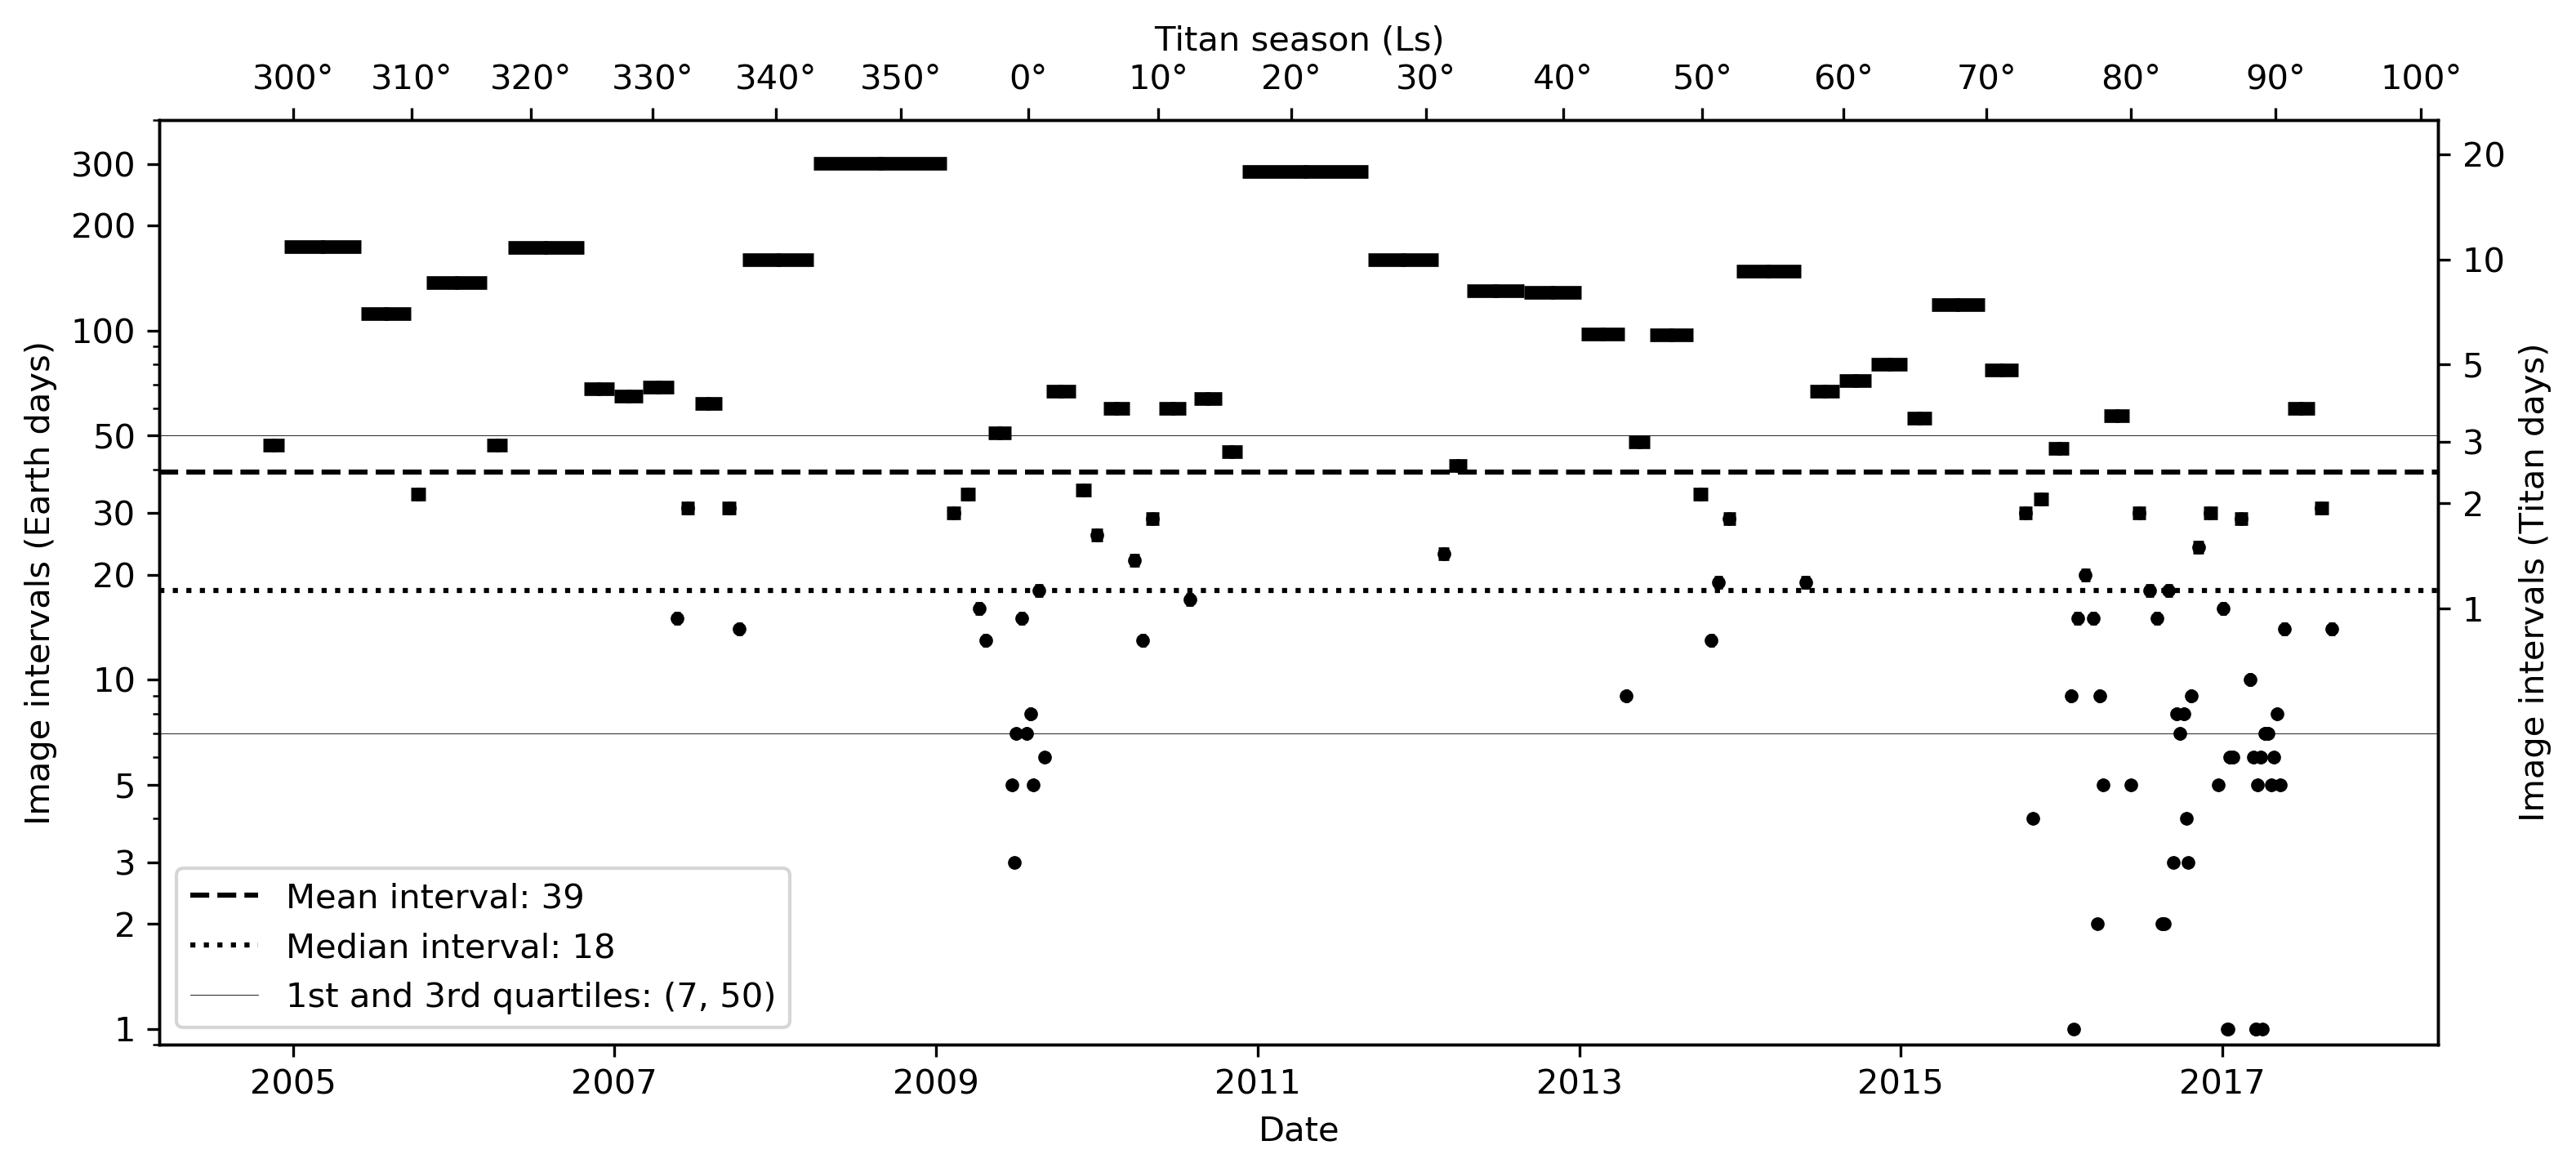
\includegraphics[width=\textwidth]{Fig2/IMG_interval.ps}
\caption{Box plot of number of Earth days between consecutive ISS/NAC CL1-UV3 observations analyzed. In average 
an image is sampled every 40 days with a range between 1 and 302 days.}
\label{fig:img_sampling} 
\end{figure}

The selected images are calibrated using the CISSCAL routines (v3.8) provided on the Planetary Data System. To improve 
the signal to noise ratio on the limb profile, we deconvolved the images with a Poisson Maximum a posteriori method 
(PMAP) using the point spread function (PSF) calculated in-flight \citep{West2010}. The image navigation are 
initialized with the spice kernel routines and the location of the center of Titan is refined by searching the maximum 
of flatness at iso-incident on the limb.  

The intensity profiles are extracted every \ang{5} bins, on both sides of the limb. Depending on the location of the 
latitude of the Sub-Cassini point on the ground, the sampling in latitude is not evenly distributed for each image.
Geometrically, the polar latitudes are less covered than the equator. The illumination also change drastically during the 
season between the northern mid-winter to summer, which restricts our ability to see both poles at the same time.


%--------------------------------------------------------------------------------------|
\subsection{Model of scattering at the limb}

To retrieve the haze extinction profiles from the I/F observations, we first model the synthetic radiance factor ($I/F$) 
with a single scattering ray tracing model in a spherical shell geometry. The effect of the multiple scattering is
accounted as a correction with a factor $\varrho_k\left(z\right)$ applied to the volume scattering along line of sight. 
This technique was used successfully several time before (e.g.,\cite{Rages1983, Rannou1997, Seignovert2016, West2018}).

In the detached layer, the multiple scattering is mainly produced by the light coming from the atmosphere below. To 
evaluate $\varrho_k$, the scattering properties of the atmosphere are fixed once for all with a setup that allows to 
reproduce the observed intensity of Titan in UV. With the radiative transfer model (the SHDOMPP from \cite{Evans1998}) 
we have access to the complete radiative source function at each level of the atmosphere. We are then able to compare the
intensity that is scattered in the direction of the observer from the direct sun only and from the direct sun and the diffuse 
field coming from below. $\varrho_k$ is defined as the ratio of multiple scattering to single scattering toward the observer 
for a given altitude and as a function of the incident and emergent angles. It is then calculated as a function the
altitude, the incident angle and the emergent angle and set in a look-up table \citep{West2018}.

We discretize the atmosphere in $N=60$ irregular layers of various thickness : $\Delta z =$ {50} {km} from the 
ground to {200} {km}, $\Delta z =$ {10} {km} from {300} to {400}{km} and from {550} to {700} {km}. Finally, we used 
$\Delta z$= {5} {km} between {400} and {550} {km}. This grid allows us to fully take advantage of the spatial resolution 
of the ISS NAC camera in the region of interest, where is the DHL. We write the outgoing radiance factor $I/F\ (z)$ as:

\begin{equation}
I/F\ (z) = \sum_{i=0}^{n_x-1} \int\limits_{x_k}^{x_{k+1}}
\frac{\left< \varpi P(\Theta) \right>_k} {4}
^{-\left( \tau^i_k\left(z\right) + \tau^e_k\left(z\right) \right)}
\beta_k\left(z\right) \varrho_k\left(z\right) d{x}
\label{eq:west2017_sup_limb}
\end{equation}

where the summation is performed on the $n_x-1$ segments defined by the intersections of the line of sight and the 
spherical shells boundaries. The impact factor $z$ (the lowest altitude reached by the line of sight) is given by the 
bottom of the $n^\mathrm{th}$ layer crossed. Therefore, each layer of the atmosphere is crossed twice. $x$ is the 
abscissa along the line of sight. $\tau^i_k$ and $\tau^e_k$ are the opacities along the incident and emergent paths. 
$\left< \varpi P(\Theta)\right>_k$ is the average of the product between the single scattering and the phase function 
at the scattering angle of the observation $\Theta$ for the layer crossed on $x_k$.  $\beta_k(z)$ is the local 
extinction at the altitude $z$. Here, the altitude $z(x)$ is the local altitude at point of abscissa $x$ along the
line of sight. The correction factor $\varrho_k\left(z\right)$ enhances the volume scattering along the line of sight. 
We find that the multiple scattering increases the scattered intensity at the limb of Titan in UV by a ratio between 
{1.05} and {1.15}, depending on the geometry of the observation. 


\subsection{Retrieval method}

Based on our previous works \citep{Seignovert2017, West2018}, we make the assumption that the optical properties 
$\left<\varpi P(\Theta)\right>_k$ of the aerosols are constant in the upper part of Titan's atmosphere. This allows 
us to focus our study only on the retrieval of the extinction along the line of sight.
% We will verify that this assumption is reasonable compared to the dynamical variability observed along the season.

In our model, an $I/F(z)$ profile only depends on the set haze extinction profile $\beta(z)$ on the geometry of 
the observation (illumination, viewing and phase angles). We assume no horizontal inhomogeneity in the atmosphere 
properties along the line of sight \citep{Seignovert2017}. We retrieve a set of extinction values $\beta_i$ (composing 
the vector ${\beta}$), with $i$ the indices of the layers, that matches the values of the radiance factor, I/F$[_i]$ 
(composing the vector {I/F}).

From the Eq. (\ref{eq:west2017_sup_limb}), it is possible to cast the scattered intensity I/F$[_i]$, as a function of 
the extinction $\beta_j$ with $j \le i$. This forms a non-linear triangular system. To find the vector ${\beta}$, we 
have to solve the formal equation:

\begin{equation}
{I/F} = {G}({\beta})
\end{equation}

where the ${G}$ is a nonlinear function which depends on the values $\beta_i$ and on the geometry of the observation.  
We could solve this system with a standard onion peeling technique and accounting for the error due to the observation 
and to the propagation of error caused, at a given level, by the errors on the $\beta_j$ in the layers above ($j<i$). 
Instead, we decided to solve the system by minimizing the difference between the modelled  $I/F$ and the observations 
using a Levenberg-Marquardt minimization. We then retrieve simultanously all the values $\beta_i$, but only the layers $i$ 
for which the tangential opacity along a line of sight ($\tau_{los}$) is small enough have an influence on the value 
of I/F$[_i]$. When $\tau_{los}$ exceeds 3, we consider that the atmosphere is too opaque and beyond this threshold we 
do not retrieve the value of $\beta$.


%--------------------------------------------------------------------------------------|
\section{Seasonal cycle of the haze extinction}


In order to provide a detailed explanation of the complex latitudinal variability of the detached haze layer, we present
some of the key images that we have analyzed. \textcolor{red}{The complete set of analyzed images should be displayed 
in appendix, I think}. From the previous work about the evolution of the detached haze in the equatorial region \citep{West2018}, 
we can define four different phases for the evolution of the detached haze layer. Between 2004 and 2008, the DHL 
was stable in altitude and extinction. Between 2008 and 2012, it settled, merged and finally disappeared 
in the main haze. During the period 2012-2016, the DHL was not observed and only sporadic transitory layers showed 
up. After 2016 and up to the end of Cassini mission, the DHL reappeared following a complex pattern. The complete 
survey is performed along a period of time which represents about half a Titan year. This is valuable because 
it encompasses the equinoctial transition period of 2009. For each phase, we display the altitude and latitude 
distribution of the instantaneous haze extinction retrieved from intensities at the illuminated limb of 
Titan. The same color scale is applied to all the panels in order to keep a consistent view on the whole dataset. 
Locations where no data are available are left as blank areas on the panels. For each map, we also display extinction 
and radiance factor vertical profiles at 4 or 5 latitudes. This provides a complementary view on the dynamics of the 
haze layers.

%--------------------------------------------------------------------------------------------
\subsection{Period 1 : Stable detached haze Layer during the Northern Winter (2004-2008) -- $L_s=$\ang{300}$-$\ang{340}} 

At its arrival in the Saturnian system in 2004, Cassini observed a single haze layer at {500} {km} 
({\bf Fig.}~\ref{fig:dhl_lat_2004_oct}) similar to the one observed at {350} {km} by Voyager 24 years before 
\citep{Smith1981}. At that moment, we were two years after the winter solstice in the northern hemisphere. In
the southern hemisphere, the haze layer is completely detached from the main haze. The haze extinction is at least 
3 orders of magnitude smaller inside the depleted zone than in the main and the detached hazes. Between the equator 
and up to about 60$^o$N it presents only a local depletion in extinction of a factor 10. There, the separation with 
the main haze is not as neat as in the south, but is still significant to defined a detached haze layer. The altitude 
of the depletion zone decreases by about {50} {km} between latitude 30$^o$N  and 60$^o$N. The detached haze layer 
merges with the polar hood beyond 60$^o$N. This description of the detached haze layer at the beginning
of Cassini mission is very consistent with the results obtained from stellar occulation in 2003 \citep{Sicardy2006}.  
In all this period between 2004 and 2008 (Ls={295}-{337}$^o$), the detached haze layer is quite stable in shape and 
is set at a constant altitude, with a maximum of extinction at {500 $\pm$ 20} {km}. The top of the main haze layer 
remains located around {450$\pm$ 20} {km} below 30$^o$N and drops by 50 km between 30 and 60$^o$N. 
\textcolor{red}{We should check that the apparent decrease in extinction of the DHL is not due to something else, 
as for instance, the phase angle. At some phase angles (near 0� or too close to 180�) may be the phase function
that we have choosen is not good enough and generate an bigger error - we should have the value of the phase angle 
in the caption.}.\\

%--
However, there are noticeable variations in haze extinction. Hereafter, we selected five representative observations 
of this period, ({\bf Fig.} \ref{fig:dhl_lat_2004_dec} to \ref{fig:dhl_lat_2007_oct}). During several months, the 
detached haze remained similar than for the first visit, but in December 2004 ({\bf Fig.} \ref{fig:dhl_lat_2004_dec}), 
the haze extinction was found a factor of 10 lower than previously at almost all latitudes at south of 30$^o$N, and 
about half a decade above 30$^o$N. The polarhood and the main haze are not affected by this decrease. In the following 
observations, ({\bf Fig.} \ref{fig:dhl_lat_2005_jun},\ref{fig:dhl_lat_2005_sept} and \ref{fig:dhl_lat_2006_may}), 
the detached haze was partially restored, but not with the same amount of extinction as before. Only observations in 
2007 ({\bf Fig.} \ref{fig:dhl_lat_2007_oct}) show extinctions in the detached haze layer comparable to those before 
the decrease. We note that the decrease of extinction below 370 km in the polar hood above 50$^o$N 
({\bf Fig.}~\ref{fig:dhl_lat_2006_may}) is due to an artefact of the inversion process. The stability of the large scale 
structure of the detached haze layer is related to the steady state of the large scale circulation during all the winter. 
The observation of October 2007 ({\bf Fig.} \ref{fig:dhl_lat_2007_oct}) is the last view that we have of this stable state 
before the seasonal turnover.\\

During this period, the detached haze also has a strong layering with, at some latitudes, distinct decks which are not 
continuous and rather appears as a foliation. This feature is more pronounced in some observations, for instance from 
June 2005 to May 2006, but does not shows up in October 2007, except marginally beyond 30$^o$N. The foliated detached 
haze layer has a larger geometrical thickness than before December 2004. This foliation is likely to be produced by a 
specific large scale circulation that can last several terrestrial months to one year.
\textcolor{red}{We should really check that the apparent difference in geometric thickness of the DHL is not
due to something else, as for instance, the phase angle. It could be due to a real effect of some aerosols above
the DHL which scatter in a different way than aerosols in DLH itself. Or it could be due to a deconvolution effect 
that could differ depending on the apparence of Titan as a full disk or a crescent...  }.  \\  

Some images allow to probe the dawn/dusk differences and longitudinal variations. Other sets of images, taken few hours 
apart, show the short term variations. They are discussed later in a dedicated section, but we can readily note that the 
detached haze layer exhibits significant longitudinal or diurnal variabilities that prevents us to discuss minor features 
observed in single images in too much details. The small scale features could depends on the local short term dynamics. 



\begin{figure}[!ht]
\centering
\includegraphics[width=12.cm,angle=00.]{Fig2/N1477222048_2.eps} \\
\vspace{0.5cm}
\includegraphics[width=12.cm,angle=00.]{Fig2/N1477222048_2-profiles.eps}
\caption{Analysis of the  {\bf Image N1477222048\_2} ({October 2004} {Ls=297$^o$} - Period 1) 
The upper panel shows the haze extinction ($\beta{ext}$) as a function of the latitude and the 
altitude, retrieved from observed radiance factors I/F. The color bar at the right hand side indicates the
value of the extinction. The figures at the bottom show, for several selected latitudes, the vertical 
profiles of the observed deconvoluted radiance factors I/F (green dots), the synthetic best fit of the I/F
 (red lines) and the retrieved haze extinction corresponding to the best fit of I/F (cyan lines and dots). 
The retrieved haze extinction are extractions of the map shown in the upper panel.}
\label{fig:dhl_lat_2004_oct}
\end{figure}

\begin{figure}[!ht]
\centering
\includegraphics[width=12.cm,angle=00.]{Fig2/N1481445613_1.eps} \\
\vspace{0.5cm}
\includegraphics[width=12.cm,angle=00.]{Fig2/N1481445613_1-profiles.eps}
\caption[]{Same as {\bf Fig.}~\ref{fig:dhl_lat_2004_oct}, but for the 
{\bf Image N1481445613\_1} ({December 2004} {Ls=300$^o$} - Period 1).}
\label{fig:dhl_lat_2004_dec} 
\end{figure}


\begin{figure}[!ht]
\centering
\includegraphics[width=12.cm,angle=00.]{Fig2/N1496548825_1.eps} \\
\vspace{0.5cm}
\includegraphics[width=12.cm,angle=00.]{Fig2/N1496548825_1-profiles.eps}
\caption[]{Same as {\bf Fig.}~\ref{fig:dhl_lat_2004_oct}, but for the 
{\bf Image N1496548825\_1}({June 2005} {Ls=306$^o$} - Period 1).}
\label{fig:dhl_lat_2005_jun}
\end{figure}

\begin{figure}[!ht]
\centering
\includegraphics[width=12.cm,angle=00.]{Fig2/N1506300441_1.eps}\\
\vspace{0.5cm}
\includegraphics[width=12.cm,angle=00.]{Fig2/N1506300441_1-profiles.eps}
\caption[]{Same as {\bf Fig.}~\ref{fig:dhl_lat_2004_oct}, but for the 
{\bf Image N1506300441\_1}({September 2005} {Ls=310$^o$} - Period 1).}
\label{fig:dhl_lat_2005_sept}
\end{figure}


\begin{figure}[!ht]
\centering
\includegraphics[width=12.cm,angle=00.]{Fig2/N1525327324_1.eps} \\
\vspace{0.5cm}
\includegraphics[width=12.cm,angle=00.]{Fig2/N1525327324_1-profiles.eps}
\caption[]{Same as {\bf Fig.}~\ref{fig:dhl_lat_2004_oct}, but for the
{\bf Image N1525327324\_1}({May 2006} {Ls=318$^o$} - Period 1).}
\label{fig:dhl_lat_2006_may}
\end{figure}

\begin{figure}[!ht]
\centering
\includegraphics[width=12.cm,angle=00.]{Fig2/N1571476343_1.eps} \\
\vspace{0.5cm}
\includegraphics[width=12.cm,angle=00.]{Fig2/N1571476343_1-profiles.eps}
\caption[]{Same as {\bf Fig.}~\ref{fig:dhl_lat_2004_oct}, but for the
{\bf Image N1571476343\_1}({October 2007} {Ls=337$^o$} - Period 1).}
\label{fig:dhl_lat_2007_oct}
\end{figure}

\subsection{Period 2 : Drop and disappearance of the main haze layer around the Vernal 
Equinox (2008-2012) -- $L_s=$\ang{343}$-$\ang{31}} 

A precursor sign of the drop of the detached haze can be seen in March 2008 ({\bf Fig.}~\ref{fig:dhl_lat_2008_mar}). 
The main haze starts an initial contraction, perceptible around around 35$^o$S. There the depleted zone is almost 
{75} {km} thick at its maximum. In January 2009, the main haze continued to fall down from {425} {km} down to {375} 
{km}  while the detached haze layer remained around {500} {km} ({\bf Fig.} \ref{fig:dhl_lat_2009_jan}). After the drop 
of the main haze in early 2009, the detached haze starts its own descent in June 2009, just before the equinox. This
delay in collapse increased the apparent thickness of the depletion zone between the two haze layers. \\

As for the main haze, the detached haze collapses first in the South hemisphere, from 500 km to 425 km, and 
then at equator and in the northern hemisphere. This is associated to the circulation turnover affecting first the
summer hemisphere ascending branch. With time, the detached haze gradually settled in altitude and finally merged with 
the main haze. The complete collapse of the detached haze is displayed in {\bf Fig.} \ref{fig:dhl_lat_2009_jun} to 
{\bf Fig.} \ref{fig:dhl_lat_2012_feb}. We note that the extinction of the detached haze is smaller at equator than at 
other latitudes, and this will be the case during all the drop. \\


\begin{figure}[!ht]
\centering
\includegraphics[width=12.cm,angle=00.]{Fig2/N1585329510_1.eps} \\
\vspace{0.5cm}
\includegraphics[width=12.cm,angle=00.]{Fig2/N1585329510_1-profiles.eps}
\caption[]{Same as {\bf Fig.}~\ref{fig:dhl_lat_2004_oct}, but for the 
{\bf Image N1585329510\_1} ({March 2008} {Ls=343$^o$} - Period 2).}
\label{fig:dhl_lat_2008_mar}
\end{figure}

\begin{figure}[!ht]
\centering
\includegraphics[width=12.cm,angle=00.]{Fig2/N1611563556_1.eps} \\
\vspace{0.5cm}
\includegraphics[width=12.cm,angle=00.]{Fig2/N1611563556_1-profiles.eps}
\caption[]{Same as {\bf Fig.}~\ref{fig:dhl_lat_2004_oct}, but for the 
{\bf Image N1611563556\_1} ({January 2009} {Ls=353$^o$} - Period 2).}
\label{fig:dhl_lat_2009_jan}
\end{figure}

\begin{figure}[!ht]
\centering
\includegraphics[width=12.cm,angle=00.]{Fig2/N1624878914_1.eps} \\
\vspace{0.5cm}
\includegraphics[width=12.cm,angle=00.]{Fig2/N1624878914_1-profiles.eps}
\caption[]{Same as {\bf Fig.}~\ref{fig:dhl_lat_2004_oct}, but for the 
{\bf Image N1624878914\_1} ({June 2009} {Ls=359$^o$} - Period 2).}
\label{fig:dhl_lat_2009_jun}
\end{figure}

\begin{figure}[!ht]
\centering
\includegraphics[width=12.cm,angle=00.]{Fig2/N1628820904_1.eps} \\
\vspace{0.5cm}
\includegraphics[width=12.cm,angle=00.]{Fig2/N1628820904_1-profiles.eps}
\caption[]{Same as {\bf Fig.}~\ref{fig:dhl_lat_2004_oct}, but for the 
{\bf Image N1628820904\_1} ({August 2009} {Ls=0$^o$} - Period 2).}
\label{fig:dhl_lat_2009_aug}
\end{figure}

\begin{figure}[!ht]
\centering
\includegraphics[width=12.cm,angle=00.]{Fig2/N1642241301_1.eps} \\
\vspace{0.5cm}
\includegraphics[width=12.cm,angle=00.]{Fig2/N1642241301_1-profiles.eps} 
\caption[]{Same as {\bf Fig.}~\ref{fig:dhl_lat_2004_oct}, but for the 
{\bf Image N1642241301\_1} ({January 2010} {Ls=6$^o$} - Period 2).}
\label{fig:dhl_lat_2010_jan}
\end{figure}

\begin{figure}[!ht]
\centering
\includegraphics[width=12.cm,angle=00.]{Fig2/N1659989492_1.eps} \\
\vspace{0.5cm}
\includegraphics[width=12.cm,angle=00.]{Fig2/N1659989492_1-profiles.eps}
\caption[]{Same as {\bf Fig.}~\ref{fig:dhl_lat_2004_oct}, but for the 
{\bf Image N1659989492\_1} ({August 2010} {Ls=13$^o$} - Period 2).}
\label{fig:dhl_lat_2010_aug}
\end{figure}

\begin{figure}[!ht]
\centering
\includegraphics[width=12.cm,angle=00.]{Fig2/N1694250019_1.eps} \\
\vspace{0.5cm}
\includegraphics[width=12.cm,angle=00.]{Fig2/N1694250019_1-profiles.eps} 
\caption[]{Same as {\bf Fig.}~\ref{fig:dhl_lat_2004_oct}, but for the 
{\bf Image N1694250019\_1} ({September 2011} {Ls=26$^o$} - Period 2).}
\label{fig:dhl_lat_2011_sep}
\end{figure}

\begin{figure}[!ht]
\centering
\includegraphics[width=12.cm,angle=00.]{Fig2/N1708076255_1.eps} \\
\vspace{0.5cm}
\includegraphics[width=12.cm,angle=00.]{Fig2/N1708076255_1-profiles.eps}
\caption[]{Same as {\bf Fig.}~\ref{fig:dhl_lat_2004_oct}, but for the 
{\bf Image N1708076255\_1} ({February 2012} {Ls=31$^o$} - Period 2).}
\label{fig:dhl_lat_2012_feb}
\end{figure}

% ({\bf Fig.} \ref{fig:dhl_lat_2009_jun} to \ref{fig:dhl_lat_2012_feb}). 
% ({\bf Fig.} \ref{fig:dhl_lat_2009_aug})
% ({\bf Fig.} \ref{fig:dhl_lat_2010_jan})  
% ({\bf Fig.} \ref{fig:dhl_lat_2012_feb})

During the fall, a second thin detached haze layer, at planetary scale, can be remarked above the collapsing detached 
haze layer. In January 2010 ({\bf Fig.} \ref{fig:dhl_lat_2010_jan}), the detached is now around {375} and {400} {km}. 
We still can see a double deck of haze, and this time the detached haze appears higher at equator than in the two 
hemispheres, producing an arch. The haze extinction has globally increased by a factor of two due to sedimentation 
in denser layers.\\

In August 2010 ({\bf Fig.} \ref{fig:dhl_lat_2010_aug}), one year after equinox, the detached haze layer continued
its drop down to {350} {km} at $\pm$ 40$^o$N and {370--400} {km} around equator. It has gained in complexity with
multiple secondary layers up to 520 km. The detached haze form a remarkable arch with a difference of about 50 km 
in altitude between the equator and the poles. This observation and the next one correspond to the same time of the
year than the time of Voyagers flybys (Ls={8$^o$} and Ls={18$^o$}). They can be compared quite directly. We now know 
that this season was a time of rapid change, and that the Voyager probes observed transient situations. Voyager also 
observed the detached haze higher near equator than elsewhere \citep{Rages1983, Rannou2000}. This corresponds to 
the detached haze layer following an isobar level.\\ 

The next observation was made in September 2011 ({\bf Fig.} \ref{fig:dhl_lat_2011_sep}). The detached haze layer is 
now well below the level of the polarhoods. Again secondary detached layers show up as high as {470} and {520} km. 
The south polarhood was not present in January 2010 ({\bf Fig.} \ref{fig:dhl_lat_2010_jan}), it could not be seen 
neither northward to 70$^o$S in August 2010 ({\bf Fig.} \ref{fig:dhl_lat_2010_aug}). We conclude that it was surely 
built in less than 20 months, and may be less than seven months. The circulation started to reverse around the equinox 
and the southward circulation send haze in the south pole and produced this polarhood. The change in haze distribution 
is a very good indication of the timing of the equinoctial circulation turnover, has it is discussed later. We note 
that the strong haze depletion at 300 km and between 30$^o$S and 20$^o$N is real but may be exagerated at 20$^o$N 
due to the limit of the retrieval procedure. The strong depletion between 250 and 300 km and between 60$^o$S and 40$^o$S 
is clearly spurious.\\ 

The last image that we have with the detached is February 2012 ({\bf Fig.} \ref{fig:dhl_lat_2012_feb}). At that 
time, the initial detached haze has completely disappeared and the secondary detached hazes is still descending
and reach {400} {km}. The secondary detached hazes is not well delineated by a layer strongly depeleted in aerosols. 
The south polarhood increases its latitudinal extent northward to 50 $^o$S and becomes larger than the northern 
polarhood which tends to decrease.  

\subsection{Period 3 : Absence of DHL with sporadic transitory layers after the Northern Spring Equinox (2012-2015) (Ls={32}-{75}$^o$)} 

During this period, the main haze layer has large scale structures which slowly evolve under the influence of the 
large scale circulation. During this period, the south and north polarhoods are still visible and they evolve
with time. Superimposed to this background haze, transient structures show up and disappear from one observation 
to the other. At some moments, large scale detached hazes appear. They differ from the detached haze seen at the 
beginning of the mission because they are not stable in time and in altitude. They do not appear from one 
observation to the other. The haze during this period is displayed in {\bf Fig.} \ref{fig:dhl_lat_2012_apr} 
to {\bf Fig.} \ref{fig:dhl_lat_2015_oct}.  \\ 

\begin{figure}[!ht]
\centering
\includegraphics[width=12.cm,angle=00.]{Fig2/N1713617586_2.eps} \\
\vspace{0.5cm}
\includegraphics[width=12.cm,angle=00.]{Fig2/N1713617586_2-profiles.eps}
\caption[]{Same as {\bf Fig.}~\ref{fig:dhl_lat_2004_oct}, but for the 
{\bf Image  N1713617586\_2} ({April 2012} {Ls=32$^o$} - Period 3).}
\label{fig:dhl_lat_2012_apr}
\end{figure}

\begin{figure}[!ht]
\centering
\includegraphics[width=12.cm,angle=00.]{Fig2/N1736054535_1.eps} \\
\vspace{0.5cm}
\includegraphics[width=12.cm,angle=00.]{Fig2/N1736054535_1-profiles.eps}
\caption[]{Same as {\bf Fig.}~\ref{fig:dhl_lat_2004_oct}, but for the 
{\bf Image N1736054535\_1} ({January 2013} {Ls=41$^o$} - Period 3).}
\label{fig:dhl_lat_2013_jan}
\end{figure}

\begin{figure}[!ht]
\centering
\includegraphics[width=12.cm,angle=00.]{Fig2/N1786775631_1.eps} \\
\vspace{0.5cm}
\includegraphics[width=12.cm,angle=00.]{Fig2/N1786775631_1-profiles.eps}
\caption[]{Same as {\bf Fig.}~\ref{fig:dhl_lat_2004_oct}, but for the 
{\bf Image N1786775631\_1} ({August 2014} {Ls=60$^o$} - Period 3).}
\label{fig:dhl_lat_2014_aug}
\end{figure}

\begin{figure}[!ht]
\centering
\includegraphics[width=12.cm,angle=00.]{Fig2/N1824610702_1.eps} \\
\vspace{0.5cm}
\includegraphics[width=12.cm,angle=00.]{Fig2/N1824610702_1-profiles.eps}
\caption[]{Same as {\bf Fig.}~\ref{fig:dhl_lat_2004_oct}, but for the 
{\bf Image N1824610702\_1} ({October 2015} {Ls=73$^o$} - Period 3).}
\label{fig:dhl_lat_2015_oct}
\end{figure}

In April 2012 ({\bf Fig.} \ref{fig:dhl_lat_2012_apr}), 

the detached haze has completely disappeared, except a residual structure at 35 -- 20$^o$S, around {370} {km}. 
This relict of the last detached haze layer is almost not perceptible in the corresponding I/F profile. At other 
latitudes, we only can see a unique main haze with a marked south polarhood and a small increase of extinction above 
65$^o$N that could be the north polarhood. Sometimes, detached layers emerge from the background with large latitudinal 
extent (e.g. detached haze at 500 km {\bf Fig.} \ref{fig:dhl_lat_2013_jan}). However, they only remain for a short time 
and are not seen in the following observations.\\

In August 2014 ({\bf Fig.} \ref{fig:dhl_lat_2014_aug}) we observed a plume of aerosol between 10$^o$S and 25$^o$N, 
at 500 km. A detached haze layer seems to have spread from this plume toward the north and the south. This 
detached haze is around {500} {km}, descending to {470} {km} at 60$^o$S (and probably even southern). At the 
north, the detached haze does not extend northern than 50$^o$N and remains at {500} {km}. This indicate an
atmosphere circulation rather flowing from equator toward the south pole. The origin of these aerosols is undefined, 
but because they scatter quite efficiently, they should be of the same nature than the aerosols of the previous 
detached haze or the main haze. The most probable is an injection from lower layers by a transient circulation. 
This structure also vanished rapidely after several months without sedimenting (\textcolor{red}{How do we know
that ???}). \\

The observation of  October 2015 ({\bf Fig.} \ref{fig:dhl_lat_2015_oct}) is very representative of the haze layer in 
the period between 2012 and the end of 2015. At this date, the main haze has a uniform scale height of {45} {km} and 
with a homogenous extinction at the planetary scale.\\   

\subsection{Period 4 : Reappearance of a new detached haze layer around the Summer Solstice : 2015-2017 (Ls={75}-{95}$^o$)} 

The first occurence of the detached haze in this period is the 3$^{rd}$ December 2015. Strictly speaking, it 
does not differ from the previous sporadic detached haze layers oberved in the period 2012 -- 2015. But, after 
this observation, the detached haze was present in each observations. The detached haze became stable in time, 
similarly to the detached haze before the equinox. Therefore, we consider this date as the beginning of the 
reappearance of the detached haze. The haze during this period is displayed in 
{\bf Fig.} \ref{fig:dhl_lat_2016_jan} to {\bf Fig.} \ref{fig:dhl_lat_2017_may}.  The observations of this period
confirms the long awaited reappearance of the detached haze layer in December 2015, just before the end of the 
Cassini mission in September 2017. 

\begin{figure}[!ht]
\centering
\includegraphics[width=12.cm,angle=00.]{Fig2/N1831867661_1.eps} \\
\vspace{0.5cm}
\includegraphics[width=12.cm,angle=00.]{Fig2/N1831867661_1-profiles.eps}
\caption[]{Same as {\bf Fig.}~\ref{fig:dhl_lat_2004_oct}, but for the 
{\bf Image N1831867661\_1} ({January 2016} {Ls=76$^o$} - Period 4).} 
\label{fig:dhl_lat_2016_jan}
\end{figure}

\begin{figure}[!ht]
\centering
\includegraphics[width=12.cm,angle=00.]{Fig2/N1850392434_1.eps} \\
\vspace{0.5cm}
\includegraphics[width=12.cm,angle=00.]{Fig2/N1850392434_1-profiles.eps}
\caption[]{Same as {\bf Fig.}~\ref{fig:dhl_lat_2004_oct}, but for the 
{\bf Image N1850392434\_1} ({August 2016} {Ls=82$^o$} - Period 4).}
\label{fig:dhl_lat_2016_aug}
\end{figure}

\begin{figure}[!ht]
\centering
\includegraphics[width=12.cm,angle=00.]{Fig2/N1856231196_1.eps} \\
\vspace{0.5cm}
\includegraphics[width=12.cm,angle=00.]{Fig2/N1856231196_1-profiles.eps}
\caption[]{Same as {\bf Fig.}~\ref{fig:dhl_lat_2004_oct}, but for the 
{\bf Image  N1856231196\_1} ({October 2016} {Ls=84$^o$} - Period 4).}
\label{fig:dhl_lat_2016_oct}
\end{figure}

\begin{figure}[!ht]
\centering
\includegraphics[width=12.cm,angle=00.]{Fig2/N1869102271_1.eps} \\
\vspace{0.5cm}
\includegraphics[width=12.cm,angle=00.]{Fig2/N1869102271_1-profiles.eps}
\caption[]{Same as {\bf Fig.}~\ref{fig:dhl_lat_2004_oct}, but for the 
{\bf Image N1869102271\_1} ({March 2017} {Ls=89$^o$} - Period 4).}
\label{fig:dhl_lat_2017_mar}
\end{figure}

\begin{figure}[!ht]
\centering
\includegraphics[width=12.cm,angle=00.]{Fig2/N1874779268_1.eps} \\
\vspace{0.5cm}
\includegraphics[width=12.cm,angle=00.]{Fig2/N1874779268_1-profiles.eps}
\caption[]{Same as {\bf Fig.}~\ref{fig:dhl_lat_2004_oct}, but for the 
{\bf Image N1874779268\_1} ({May 2017} {Ls=91$^o$} - Period 4).} 
\label{fig:dhl_lat_2017_may}
\end{figure}

At the beginning, the detached haze layer is not very well defined but it can be perceived at all latitudes 
around 490 --  520 km ({\bf Fig.} \ref{fig:dhl_lat_2016_jan}). We notice at the same moment a contraction 
the main haze, with the top of the haze dropped by {50} {km} in January 2016 compared to October 2015. The
main elements of the reappearance (altitude and date) confirms the predictions made by the general circulation models 
\citep{Lebonnois2012,Larson2015} and the prediction reported in \cite{West2011}. The detailed comparison between 
the observations and GCM is discussed further.  \\

With time, the detached haze layer is better marked and the zone of depletion is more pronounced, especially in the 
northern hemisphere ({\bf Fig.} \ref{fig:dhl_lat_2016_aug}). The situation seems to be analogue to an early stage of 
the structure observed in 2004 (with the opposite latitude). However, although the detached haze persists in time, 
it also settles and almost merges with the main haze in September or October 2016 ({\bf Fig.} \ref{fig:dhl_lat_2016_oct}). 
In the  following observations ({\bf Fig.} \ref{fig:dhl_lat_2017_mar} and {\bf Fig.} \ref{fig:dhl_lat_2017_may}), we are 
witnessing the complex evolution of the first appeared detached haze that merge with the main layer at latitude southward 
to $\simeq$35$^o$N while it remains stable around {450} {km} northward to 35$^o$N and seems to vanish rather than settle.  \\

A secondary detached haze layer appears in the southern hemisphere at high altitude around {520} {km}
({\bf Fig.} \ref{fig:dhl_lat_2016_oct}). Its northern boundary is not well defined. This new structure will be persistent with 
time, at planetary scale up to the end of Cassini mission but is gradually descending. The results reported by \cite{West2018} 
concerns the detached haze at equator only. Although they already revealed a complex behaviour of the detached haze layer, the 
present observations show a dichotomy between the two hemispheres. The detail of the evolution, the split in a double layer 
structure, the formation and disappearance of several structures was completely unexpected. According to GCMs, six years 
after equinox, the post-equinoctial circulation was supposed to be already installed with a planetary scale circulation cell 
from the south hemisphere to the north polar region. Apparently, this is not the case.  \\ 

These observations from 2004 to 2017 does not completely cover half a Titan year. The first and last observations 
were taken almost at the opposite season, Ls=297$^o$ and 94$^o$ respectively (they are 157$^o$ apart). This prevents
direct comparisons between the detached haze at the beginning and at the end of the mission, although in both cases 
they are taken more than a season after the previous solstice, quite close from the solstices.  


%--------------------------------------------------------------------------------------|
% \section{Seasonal evolution of the depletion below the detached haze}
% 
% The equatorial extinction profile along the seasons and the location of the peak of intensity was presented 
% before in the {\bf Fig.} \ref{fig:west2017_dhl_time_eq}.   We saw in the previous section that sometimes, it is 
% difficult to define the location and the thickness of the detached haze layer (especially in the case of double 
% layers). Here, we look at the thickness of the largest depletion inside the profile as an other proxy of the
% evolution of the detached haze layer.  The {\bf Fig.} \ref{fig:seignovert2018_shl_dep_lats} summarizes its 
%thickness and its location with time.  
% 
% \begin{figure}[!ht]
% \includegraphics[width=12.cm,angle=00.]{Fig2/DHL_time-Dep.eps} 
% \caption{Summary of the location
% of the main depletion below the detached haze layer as a function of the
% time and altitude for the different latitudes (bins of {$\pm$ 5$^o$}). The
% size of the dots is proportional to the vertical thickness. The gray
% areas correspond to the periods with no data.}\label{fig:seignovert2018_shl_dep_lats2} 
% \end{figure}
% 
% Before the equinox, at all the latitude lower than 60$^o$N, the detached haze layer is well pronounced and very 
% stable in altitude at {480} {km} and in thickness ({50}{km}). During this period, the coverage above 60$^o$N is 
% sparse. The spurious occurrence of depletion highly depends on the extent of the northern polar hood. Around the 
% equinox, the depletion grows rapidly up to {100} {km} due to the contraction of the main haze. Then, just after the 
% equinox, the depletion decreases due to the fall of the detached haze layer. As noticed before, the collapse is
% quicker in the southern hemisphere compared with the equator. After the disappearance of the detached haze layer in 
% 2011. Some spurious depletion can be observed but does not form a consistent pattern and vanish rapidly. Finally, 
% in 2016, the consistent depletion emerges from 30$^o$S to the North pole at {470} {km} (like in 2004) but this time 
% with a thickness of {25} {km}. This depletion falls during the year 2016 at the same rate as the fall observed during
%  the equinox. The depletion only remain stable at {450} {km} above 60$^o$N. In 2017, the secondary layer appears at 
% {520} {km} and is visible in the extinction profiles at all the latitudes. However, the very last Cassini images of 
% May 2017 only confirmes it in the northern hemisphere.
%
%

%--------------------------------------------------------------------------------------|
\section{Local and short term variabilities of the detached haze layer}

So far, we have considered the evolution of the detached in the frame of the seasonal change.
We then discussed the long term evolution at the planetary scale. In this section, we now consider 
sets of observations which allows to characterize specific behaviour of the detached haze. We 
then choose several observations taken few hours apart to evaluate the variability of the 
detached haze layer at the scale of the hour, we consider observations at low phase angle which 
show simultaneously the two limbs of Titan, and finally, we consider observations taken from a 
near polar point of view which enable to see the longitudinal variations of the detached haze in 
a narrow range of latitudes.  

\subsection{Short time or spatial  variability}\label{sec:dhl_time_short}

As presented before, we observe between December 2004 and June 2005 a large amplitude variability of the 
detached haze layer extinction profile at all the latitudes below 35$^o$N ({\bf Fig.} \ref{fig:dhl_lat_2004_dec} 
and \ref{fig:dhl_lat_2005_jun}). Fortunately, Cassini took in June 2005 a series of 9 images of 
Titan with a time-step of {80} {minutes} appart (Table \ref{tab:dhl_lat_2005_jun_timeshort}).
With multiple observations of Titan in a short period, we are able to validate our calibration and 
to determine short time and local variability. Here, we analyze the sequence at three different 
locations on the limb (40$^o$S, 0$^o$, 40$^o$N). The 9 observations are made with  phase angles around $10^o$, 
within an interval of 0.6$^o$. The longitude of the observations varies  between 349.6$^o$E and 344.8$^o$E
and the solar local time on Titan varies between 17:12  and 17:36.\\

\begin{table}[!ht]
\centering
\caption[DHL - Short timescale variability - June 2005]{Sequence of the 9 images of Titan taken 
June 4$^\mathrm{th}$, 2005. The longitude and local time are given for the profile at the equator 
on the illuminated side of Titan.}
\small
\begin{tabular} {c c c c c}
\toprule
Imag ID & Time (UTC) & Phase & Longitude (Eq) & Local Time (Eq)\\
\midrule
N1496548825\_1 & 03h32 & 10.4 & 349.3$^o$E & 17h12 \\
N1496552665\_1 & 04h36 & 10.2 & 349.6$^o$E & 17h18 \\
N1496557465\_1 & 05h56 & 10.0 & 349.4$^o$E & 17h24 \\
N1496562265\_1 & 07h16 &  9.9 & 346.9$^o$E & 17h18 \\
N1496567065\_1 & 08h36 &  9.8 & 346.6$^o$E & 17h24 \\
N1496571865\_1 & 09h56 &  9.8 & 346.1$^o$E & 17h24 \\
N1496576665\_1 & 11h16 &  9.8 & 345.7$^o$E & 17h30 \\
N1496581465\_1 & 12h36 &  9.9 & 345.3$^o$E & 17h30 \\
N1496586265\_1 & 13h56 & 10.1 & 344.8$^o$E & 17h36 \\
\bottomrule
\label{tab:dhl_lat_2005_jun_timeshort}
\end{tabular}
\end{table}

\begin{figure}[!ht]
\centering
\includegraphics[width=12.cm,angle=00.]{Fig2/IMG_time.eps} 
\caption[DHL - Shot timescale variability - June 2005]{ Extinction profiles for the serie 
of 9 images taken {80} {minutes} apart in June 2005 (cf. Table \ref{tab:dhl_lat_2005_jun_timeshort}). 
The corresponding extinction map is shown the {\bf Fig.}\ref{fig:dhl_lat_2005_jun}.} 
\label{fig:dhl_lat_2005_jun_timeshort}
\end{figure}

The {\bf Fig.} \ref{fig:dhl_lat_2005_jun_timeshort} presents extinction profiles extracted from the analysis of the
nine images. First, we confirm that our calibration method is reliable from one picture to the other and the overall 
variability of the detached haze is very small. We clearly observe the double layering at 40$^o$S and 40$^o$N reported 
previously. All the locations of the maximum of the extinction peaks are located within a small altitude range (smaller 
than the {8} {km} of the pixel scale). Then, the vertical offsets which are observed at different times are consistent 
with  the accuracy of the georeferencing, and therefore are not significant. At the equator and at 40$^o$S, the detached 
haze layer is well detached for all the profiles. When the vertical offset is accounter for, all the extinctions are found 
with relative differences of about $\pm$ 10\% compared to the average value, except in the depletion zone between 
the main and detached haze layers where difference can reach an order of magnitude (at 0$^o$) to several order of magnitude
(40$^o$N). The variations outside the depletion zone are not significant \citep{West2018}. We note that the different behaviour 
of the N1496576665\_1 profile at 40$^o$S and below {450} {km}, compared to other profiles, is an artefact due to the inversion 
process. \\ 

The variability in the depletion zone at the equator is probably due to the retrieval uncertainties. The differences in 
extinction are about one order of magnitude, consistent with uncertainties between the two layers (e.g. \cite{West2018}),
and without specific temporal evolution. The variability observed at 40$^o$N, in the depletion zone around 460 km are significant
for two reasons. First, the differences are much larger than the expected uncertainty in this zone. Second, the sequence shows 
a gradual and consistent increase of extinction with time. If these differences were due to uncertainties in the retrieval procedure, 
it would have rather given a chaotic evolution of the extinction with time.\\

We also remark that the corresponding extinction map ({\bf Fig.}\ref{fig:dhl_lat_2005_jun}) shows that in the south, 
the detached haze is well separated from the main haze by a well defined depletion zone. In the north, the depletion 
zone is less well defined and the detached haze and the main haze are connected vertically by a residual haze.
The variation of this residual haze is the one reported in {\bf Fig.} \ref{fig:dhl_lat_2005_jun_timeshort} at 40$^o$N. 
We can not strictly determine if we are witnessing time or a spatial variations since both the time and the longitude 
of the observations change simultaneously during the image sequence. We note that a rotation of 5$^o$ in longitude corresponds 
to a maximum shift of 250 km in distance (one tenth of Titan radius), possibly consistent with a spatial variation of 
the haze extinction. \\ 


\subsection{Dusk and dawn sides}\label{sec:dhl_dusk_dawn}


\begin{figure}[!ht]
\centering
\includegraphics[width=12.cm,angle=00.]{Fig2/N1496548825_1_sides.eps} \\
\vspace{0.5cm}
\includegraphics[width=12.cm,angle=00.]{Fig2/N1496548825_1-profiles_sides.eps}
\caption[]{The two panels show the map of the haze extinction for the dusk and dawn side of 
Titan for the image {\bf Image N1496548825\_1} ({June 2005} {Ls=305$^o$}). At the bottom, three
figures show the haze extinction vertical profiles at three latitudes and for the two sides of 
Titan. At bottom and right, the image of Titan with the location along the limb where the 
profiles are taken with the same color code for dusk and dawn than for the vertical profiles.
The blue and yellow dots are the sub-spacecraft and the subsolar points respectively.} 
\label{fig:dhl_lat_2005_jun_duskdawn} 
\end{figure}

\begin{figure}[!ht]
\centering
\includegraphics[width=12.cm,angle=00.]{Fig2/N1562037403_1_sides.eps} \\
\vspace{0.5cm}
\includegraphics[width=12.cm,angle=00.]{Fig2/N1562037403_1-profiles_sides.eps}
\caption[]{Same as {\bf Fig.}~\ref{fig:dhl_lat_2005_jun_duskdawn}, but for the 
{\bf Image N1562037403\_1} ({July 2007} {Ls=333$^o$}).}
\label{fig:dhl_lat_2007_jul_duskdawn} 
\end{figure}

\begin{figure}[!ht]
\centering
\includegraphics[width=12.cm,angle=00.]{Fig2/N1624599912_1_sides.eps} \\
\vspace{0.5cm}
\includegraphics[width=12.cm,angle=00.]{Fig2/N1624599912_1-profiles_sides.eps}
\caption[]{Same as {\bf Fig.}~\ref{fig:dhl_lat_2005_jun_duskdawn}, but for the 
{\bf Image N1624599912\_1} ({June 2009} {Ls=359$^o$}).}
\label{fig:dhl_lat_2009_jun_duskdawn}
\end{figure}

\begin{figure}[!ht]
\centering
\includegraphics[width=12.cm,angle=00.]{Fig2/N1843761608_1_sides.eps} \\
\vspace{0.5cm}
\includegraphics[width=12.cm,angle=00.]{Fig2/N1843761608_1-profiles_sides.eps}
\caption[]{Same as {\bf Fig.}~\ref{fig:dhl_lat_2005_jun_duskdawn}, but for the 
{\bf Image N1843761608\_1} ({April 2016} {Ls=80$^o$}).}
\label{fig:dhl_lat_2016_apr_duskdawn}
\end{figure}


Aside from short time and local variations, we also are interested by images showing simultaneously the two sides
of Titan. This geometry of observation allows us to retrieve the haze extinction with both the illuminated and the 
dark side of Titan simultaneously  ({\bf Fig.} \ref{fig:dhl_lat_2005_jun_duskdawn} to 
{\bf Fig.} \ref{fig:dhl_lat_2016_apr_duskdawn}). In this case, we can compare the dawn and dusk part of the limb for 
specific latitudes. The dusk side is the East side of Titan which is entering into the night and the dawn side is the 
West side of Titan which is going out from the night. Although Titan's day is about 16 terrestrial days, the time spent 
by the haze into the night or at the daylight is much shorter. First, the atmosphere is superrotating and at altitude 
around 400 or 500 km the zonal wind is comparable to or larger than the rotation speed of the ground (11.7 m/s) 
\citep{Flasar2005, Lebonnois2012}. This makes the actual diurnal cycle for the high altitude hazes shorter 
than 16 days by a factor of 2 or more. The second point is that, at high altitude, the solid body of Titan masks the sun
to the haze layer less than half of the time. Thus, effects on the haze should be produced by process with timescale 
comparable with a terrestrial day. Dynamics is the most obvious process to produce inhomogeneities.\\


The {\bf Fig.} \ref{fig:dhl_lat_2005_jun_duskdawn} presents the haze extinction at the dusk and dawn sides as observed 
the June 2005 (N1496548825\_1). The detached haze differs significantly between the two sides. At the equator,
we observe a thin layer of {10} {km} in the dusk side whereas in the dawn side it appears as double detached layer 
of {40} {km} thickness. The haze extinction at the peak differs significantly, from 2.5$\times 10^{-8}$ to 
7$\times 10^{-8}$ m$^{-1}$. The depletion below the haze layer is also less pronounced in the dawn side compared to 
the dusk side. Although this observation was taken during the period of stability for the detached haze, we 
observed a significant asymmetry between the dawn and dusk side.\\

Two years later, another low phase angle image was recorded ({\bf Fig.} \ref{fig:dhl_lat_2007_jul_duskdawn}). 
This time, the detached haze layer is much more symmetrical between the two sides. The peaks of haze extinction 
are at the same altitude with comparable values. However, small differences could be noticed : there is a
small secondary layer above the detached haze at the dawn side between 50$^o$S and 20$^o$N, and may be even
northward. In the northern hemisphere, the extinction appears slighty larger at dawn that at dusk, and the 
vertical extend of the detached haze is also a bit larger. \\


At the equinox, the detached haze layer already started its drop in altitude ({\bf Fig.}~\ref{fig:dhl_lat_2009_jun_duskdawn}). 
There is significant differences between the two sides, in both hemispheres, while at the equator the two
profiles are almost identical. The haze layer is not exactly symmetrical in the southern hemisphere. The detached 
haze itself is at the same altitude, but the depletion zone is at lower altitude at the dawn side, and the main 
haze layer is thicker at the dusk side. In the northern hemisphere, the haze layer is more complex, and the 
asymmetry is even more marked with a detached haze at different altitude and with a different extinction. The 
detached and main haze layers at the dusk side appears optically thicker than the layers at the dawn side. This is 
opposite to the two previous cases.  \\ 


After the equinox, a fewer number of images were taken at low phase angle. Among them, we do not notice any 
significant differences between the dawn and dusk sides. After the reappearance of the detached haze layer in 
2016, we found only one image with the relevant geometry to see both sides of Titan illuminated at the same time 
({\bf Fig.} \ref{fig:dhl_lat_2016_apr_duskdawn}). In this case, the dark side does not provide information 
because the phase angle is too large, but the illuminated side spans all over the northern hemisphere that can
be observed twice on the bright side. The main haze appears very symmetrical in both sides and almost identical
above 50$^o$N. The depletion can be followed continuously all around the North Pole. At latitude lower than 
50$^o$N, the value of the haze extinctions are similar but the altitudes of the extinction peak different by 
{25} {km}. We also observe partial secondary detached layers in each side, but not at the same latitudes.\\ 

The haze extinction and the altitude of detached haze layer can differ significantly between the dusk 
and dawn sides. But no general rule or trend can be established to explain  these differences. Especially,
it is not possible to invoke a diurnal cycle because there is not a systematic effect. As for the short time 
variablility, we can not disantangle spatial (longitudinal) and time variations.\\   


\subsection{Longitudinal variability}\label{sec:dhl_lon}

\begin{figure}[!ht]
\centering
\includegraphics[width=12.cm,angle=00.]{Fig2/N1617163560_1_lon.eps} \\
\vspace{0.5cm}
\includegraphics[width=12.cm,angle=00.]{Fig2/N1617163560_1-profiles_lon.eps} 
\caption[]{The panels show the map of the haze extinction at a given latitude and as a function of 
the longitude and the local hour for the image {\bf Image N1617163560\_1} ({March 29, 2009} {Ls=356$^o$}). 
The color bar at the right hand side indicates the value of the extinction. The figures at the bottom show, 
for two selected latitudes, the vertical profiles of the observed deconvoluted radiance factors I/F (green 
dots), the synthetic best fit of the I/F (red lines) and the retrieved haze extinction corresponding to the
best fit of I/F (cyan lines and dots). The retrieved haze extinction are extractions of the map shown in 
the upper panel. At bottom and right, the image of Titan with the location along the limb where the profiles 
are taken The blue dot show the sub-spacecraft} 
\label{fig:dhl_lat_2009_mar_lon_29}
\end{figure}

\begin{figure}[!ht]
\centering
\includegraphics[width=12.cm,angle=00.]{Fig2/N1618568958_1_lon.eps} \\
\vspace{0.5cm}
\includegraphics[width=12.cm,angle=00.]{Fig2/N1618568958_1-profiles_lon.eps} 
\caption[]{Same as {\bf Fig.}~\ref{fig:dhl_lat_2009_mar_lon_29}, but for the 
{\bf Image N1618568958\_1} ({April 14, 2009} {Ls=356$^o$}).}
\label{fig:dhl_lat_2009_apr_lon_14}
\end{figure}

\begin{figure}[!ht]
\centering
\includegraphics[width=12.cm,angle=00.]{Fig2/N1619710966_1_lon.eps} \\
\vspace{0.5cm}
\includegraphics[width=12.cm,angle=00.]{Fig2/N1619710966_1-profiles_lon.eps} 
\caption[]{Same as {\bf Fig.}~\ref{fig:dhl_lat_2009_mar_lon_29}, but for the 
{\bf Image N1619710966\_1} ({April 29, 2009} {Ls=356$^o$}).}
\label{fig:dhl_lat_2009_apr_lon_29}
\end{figure}

% \begin{figure}[!ht]
% \centering
% \includegraphics[width=12.cm,angle=00.]{Fig2/N1849875547_1_lon.eps} 
% \vspace{0.2cm}
% \includegraphics[width=12.cm,angle=00.]{Fig2/N1849875547_1-profiles_lon.eps}
% \caption[]{Same as {\bf Fig.}~\ref{fig:dhl_lat_2009_mar_lon_29}, but for the 
% {\bf Image N1849875547\_1} ({August 2016} {Ls=82$^o$}).}
% \label{fig:dhl_lat_2016_aug_lon}
% \end{figure}

Observations of Titan taken from a near polar point of view offer a unique way to study the evolution of 
the detached haze with a large coverage in longitude and within in a small range of latitudes. It allows 
first to check the homogeneity of the haze in longitude, and it also allows us to extent our previous 
observations between the dusk/dawn sides with a continuous coverage from 6:00 to 18:00.\\

We could analyze a set of three images taken sequentially. The first observation was performed the 
29$^{th}$ of March 2009 ({\bf Fig.} \ref{fig:dhl_lat_2009_mar_lon_29}) during the collapse of the detached 
haze layer. Two other observations were made only two weeks and one month later, with the same geometry 
({\bf Fig.} \ref{fig:dhl_lat_2009_apr_lon_14}, \ref{fig:dhl_lat_2009_apr_lon_29}). The detached haze layer is 
located at {470} {km} at all the longitudes. Inside the depletion region, we notice a plume of haze 
between {400} and {440} {km} and between 140$^o$E and 210$^o$E. In mid-April, the plume is located between
120$^o$E and 200$^o$E between {375} and {425} {km} and appears disconnected and settling from the detached 
layer, which remains at {470} {km}. At the end of April, we now see the extension around {410} {km} and it 
is spread from 110$^o$E and 180$^o$E. This separated aerosols plume is now connected with the main haze.\\ 

This feature is not correlated with the local time but remains about at the same longitude and drifts slowly 
toward the West. This would correspond to a retrograde motion of about 0.6 m/s. Another solution would be 
prograde motion of 6.6 m/s, in phase with the sampling of 15 terrestrial days. The vertical speed, assuming
that the aerosol cloud drop from 400 km to 375 km in one month would be $10^{-3}$ m/s. We also can remark a 
modulation in the extinction and in the geometrical thickness of both the detached haze layer and the main 
haze. By comparing the three observations, we find that they are not directly linked to a common local time.
In the last image, only the geometrical thickness is modulated and not the haze extinction. \\

% Another observation with a polar viewing was performed in August 2016 ({\bf Fig.} \ref{fig:dhl_lat_2016_aug_lon}). 
% That time, the latitude also varies from 30$^o$N at 180$^o$E to 50$^o$N at 240$^o$E and return to 30$^o$N 
% 300$^o$E. The depletion below the detached layer is slightly more pronounced between 180$^o$E and 240$^o$E and 
% the top of the main haze varies. And the top of main haze layer has also variations. For this observation, 
% we do not observe strong longitudinal variation.  \\

These observations show that the haze layer is not completely homogeneous in longitude and have important 
fluctuations in extinction and in geometry (\textcolor{red}{NB : I think that the curve  $\beta_{max}$ 
.vs. Longitude and Thickness .vs. Longitude would be useful here to have a quantitative view on these
variations. At least, we should give an numerical value for the order of magnitude of these variations in 
the DHL}). It also strenghten the idea that space and time 
variations, as in observations previously discussed, can not be distinguished with so few data. The dawn/dusk 
differences and the short term variations, presented in the two previous subsections, could be due to longitudinal 
effect rather than to time to time variations. Therefore, with the results of this section, we stress that the 
longitude inhomogeneities should be kept in mind when discussing and comparing latitudinal maps of detached haze layer.


% The study of the longitudinal variabilities of the detached layer requires flyby over the polar region. This geometry 
% is only encountered a few times during the whole Cassini mission. No heavy trend is found concerning longitudinal 
% variation, but we showed that the detached haze is not completely homogeneous in longitude and some marked structures    
% exist only at some longitudes. This is the case for the detached cloud in the depleted region and for the modulation 
% of the detachez haze thickness observed between the 29 March and 29 April 2009. On the other hand, the 16 August 2016, 
% the detached was fairly homogeneous. Finally, the dusk/dawn effect reported previously is not observe in this subset. 
% Therefore we can hardly generalize these results. We can only stress that the longitude inhomogeneities should be kept 
% in mind when discussing and comparing latitudinal maps of detached haze layer retrieved within narrow ranges of longitude. 

%--------------------------------------------------------------------------------------|

\section{Comparison between our results and retrieval from UVIS instrument and with GCM predictions}\label{sec:dhl_comparaisons2} 

The extinction profiles retrieved in the previous sections can be compared with results obtained with other
instruments, such as UVIS when the altitude is higher than {450} {km} \citep{Koskinen2011}.
%and CIRS for the lower part from {400} to {300} {km} \citep{Vinatier2015}. 
For both instruments, only a limited number of latitude profiles can be used to compare with our results.

\subsection{Comparison with UVIS results above {450} {km}}

\cite{Koskinen2011} performed a complete analysis of the mesosphere and thermosphere of Titan using UVIS stellar
occultations. The sensitivity of UVIS during a stellar occultation is much better than what ISS can achieve. However, 
while ISS probes the light scattered by the detached haze layer, UVIS probes the light transmitted through a tangential 
path at the limb. In both cases, an extinction profile can be retrieved. ISS can only retrieve the extinction of the 
particles which scatters light, and under assumptions concerning the phase function and the single scattering albedo. 
On the other hand, UVIS is able to retrieve the total extinction from transmission with no assumption about the haze 
particles. In theory, this difference is valuable because it would give a unique information about the change in aerosol 
size with altitude. In practice, ISS sensitivity is not sufficient to reach the requested sensitivity to probe above 
the peak of the detached haze by more than a scale height. 

Two of the UVIS occultation profiles, in 2008 and 2009 (T41 and T53 flybys), can be compared to ISS observations at 
the same location and at the same period ({\bf Fig.} \ref{fig:dhl_comp_uvis}). The UVIS profiles are scaled to
offset the spectral dependance between ISS and UVIS effective wavelength (338 and 190 nm respectively). This difference
is due to the spectral dependance of the extinction cross-sections and to the intrinsic differences arising from
comparing the extinction retrieved from scattering properties or from occultation \citep{Cours2011}. 

\begin{figure}[!ht]
\centering
\includegraphics[width=12.cm,angle=00.]{Fig2/ISS_UVIS-Haze.eps}
\caption[UVIS comparison]{Comparison between ISS and UVIS extinction profiles before the equinox. UVIS profiles are 
retrieved by \cite{Koskinen2011} during the T41 (2008/02/23) and T53 (2009/04/19) flybys. ISS profiles are retrieved 
for the images N1585329510\_1 (2008/03/27) and N1618568958\_1 (2009/04/16). The UVIS profile are scaled by a factor {0.15} 
to compensate the spectral dependance of the extinction cross section and overlap ISS retrievals.}
\label{fig:dhl_comp_uvis}
\end{figure}

The comparisons between the two extinction profiles show a very good match between the two extinction profiles below 
between {450} and {550} {km}. Considering that UVIS and ISS profiles are not taken exactly at the same date and
at the same longitude, the results of the previous section demonstrate that these differencess are consistent with 
the natural variabilities observed in the detached haze layer. This comparison is then a good validation of our
results concerning the extinction profiles of the detached haze.\\ 

Above {575} {km}, UVIS extinction profiles show the presence of a secondary layer at {610} {km} which is not detected 
by ISS. As shown by \cite{Cours2011}, ISS is only sensitive to the larger aerosols, those that scatter light, whereas 
UVIS is able to probe the extinction of all the particules, and especially the smaller ones which do not scatter. 
In theory, the difference between UVIS and ISS above {575} {km} may reveal a sharp change in aerosol size distribution.
But, this layer is located at altitudes where the signal to noise is low and structure may be erased during the 
deconvolution. Therefore, it is not possible to draw safe conclusion from the profiles above {575} {km}.\\


\subsection{\textcolor{blue}{Comparaison with CIRS results below {400} {km}}} 

\begin{figure}[htbp]
\centering
\includegraphics[width=12.cm,angle=00.]{Fig2/ISS_CIRS-Haze_2010-06.eps} 
\vspace{0.2cm}
\includegraphics[width=12.cm,angle=00.]{Fig2/ISS_CIRS-Haze_2011-06.eps}
\vspace{0.2cm}
\includegraphics[width=12.cm,angle=00.]{Fig2/ISS_CIRS-Haze_2012-07.eps}
\vspace{0.2cm}
\includegraphics[width=12.cm,angle=00.]{Fig2/ISS_CIRS-Haze_2012-11.eps}
\caption[CIRS comparison]{\textcolor{blue}{Comparison between ISS and CIRS \citep{Vinatier2015} extinction profiles. The CIRS profiles 
are scaled by a factor {500} to compensate the spectral dependance of the extinction cross section \citep{Vinatier2012} 
and in order to be compared with ISS retrievals. In June 2011, the ISS profile is shifted upward (dashline) to provide 
a better correspondance of the observed depletion.}} 
\label{fig:dhl_comp_cirs}
\end{figure}
 
\textcolor{blue}{
CIRS is sensitive to the thermal emission of the stratosphere and the mesosphere where is located the main haze. The 
aerosols thermal signature is very complex due to their high polymerization and is difficult to extract from the continuum
\citep{Vinatier2010}.  However, \cite{Vinatier2015} provided a series of extinction profiles for the haze just after the 
equinox between June 2010 and November 2012. We extracted the extinction profiles derived with ISS at the same location 
during the same period ({\bf Fig.} \ref{fig:dhl_comp_cirs}) and scaled them to compensate the spectral dependance of the 
extinction cross-section using \cite{Vinatier2012}. The comparison between the results of the two instruments is not
very easy for several reasons : first, we only consider UV observations of ISS which probes the top of the haze 
layer above 300 km and CIRS probes the haze layer between 150 km and 400 km. Only a moderate part of the haze layer, 
between about 300 and 400 km, is probed by both instruments. Second, the vertical  resolution of CIRS profiles is 
between 30 and 50 km. The extinction obtained with CIRS correspond to averaged values on altitude range comparable
to this sampling. Inside the altitude range in common between ISS ans CIRS, 3 to 5 values of extinction are produced 
by CIRS. This make comparisons difficult.  }

\textcolor{blue}{
Just after the equinox in June 2010, we obtain some agreements between the CIRS and the ISS extinction profile below 
{400} {km} ({\bf Fig.} \ref{fig:dhl_lat_2010_aug}). The depletion below the detached haze laze layer is located at 
{350}{km} in both profile and for all the southern latitudes. The variability of the depletion is much more important 
with CIRS than with ISS ({\bf Fig.} \ref{fig:dhl_lat_2010_aug}). However during this period the detached haze layer 
evolves rapidly and its structure in the northern hemisphere is very complex with multiple sub-layers inside the
depression.  }

\textcolor{blue}{
A year later, in June 2011, we observe a discrepancy between the two retrievals. Originally the profiles seemed to be in 
anti-phase but when we shift the ISS profiles by only {30} {km} upward, we obtain a better agreement between both 
instruments. According to Sandrine \textsc{Vinatier}, CIRS data are well corrected after the calibration in altitude and 
should be less affected than ISS by the drift of the kernels. Moreover, at this specific period, the whole upper 
atmosphere is affected by the change of season and the collapse of the detached haze. It could be likely that our 
navigation with iso-incidence method failed by a couple of pixels in this case ({\bf Fig.} \ref{fig:dhl_lat_2011_sep}). If 
it is the case, this will move upward all the equatorial region even more than what was reported.  }

\textcolor{blue}{
In July 2012, CIRS detects a double depletion when ISS only see a single scale height up to its saturation point at 
{350} {km}. Above {400}{km} the CIRS data could be subject to large uncertainties (\textsc{Vinatier} personal 
communication) and should not be taken for granted. In the small common region, the scale height is the same even if the 
intensity does not align. The match in intensity is a bit better in November. For both dates, the depletion observed by 
CIRS is out of reach from ISS but could be the continuity of the descent of the detached haze layer inside the main haze 
(as suggested in the {\bf Fig.} \ref{fig:dhl_lat_2011_sep}, \ref{fig:dhl_lat_2012_feb}). To confirm this assumption we
will need to probe the lower part of the atmosphere with other filters.
}

\textcolor{blue}{
As reported by \cite{Vinatier2016}, a lower mass mixing ratio is observed by CIRS in January 2016 at {400} {km} in the
northern hemisphere.  This results matchs perfectly the location of the depletion observed by ISS at the same moment in
the same region ({\bf Fig.} \ref{fig:dhl_lat_2016_jan}). More cross analysis needs to be done during this recent period to 
drive further conclusions.  
}

\textcolor{red}{BENOIT : I do not understand everything about the comparison with CIRS : 1) You only
selected few vertical profiles at some latitudes in CIRS data (with which criterions ?) although CIRS results are 
displayed as panels, similarly to ISS. 2)  Since CIRS has latitude/altitude panels, these should be the kind of things
we should compare... I think we would immediately  notice that there is nothing to compare because the regions which 
are probed by the two instrument (at least in UV for ISS) are totally different and the overlap (between 300 and 
400 km) is to narrow for a useful comparison. 3) Comparisons between ISS and CIRS should be performed with ISS data
at larger wavelengths, where the region which are probed are much deeper, as you displayed in your PhD report. I 
propose then to remove this part (above in blue) from the paper since it brings almost nothing} 


\subsection{Comparison with general circulation models}

\begin{figure}[!ht]
\centering
\includegraphics[width=7.cm,angle=00.]{Fig2/Lebonnois2012_Fig4_winter.eps} 
\includegraphics[width=7.cm,angle=00.]{Fig2/Larson2015-Fig7_Winter.eps}
\vspace{0.5cm}
\includegraphics[width=12.cm,angle=0.]{Fig2/N1477222048_2-all.eps} 
\caption[GCM extinction in winter]{At the top, the zonally averaged haze extinction at the Northern Winter Solstice 
(Ls={270$^o$}) estimated by \cite{Lebonnois2012} at the wavelength $\lambda=${700} {nm} (left) and by \cite{Larson2015} 
at $\lambda=${525} {nm} (right). At the bottom, haze extinction map retrieved from Cassini/ISS observation CL1-UV3
($\lambda=${340}{nm}) in the middle of the winter (Ls={300$^o$}, Image N1477222048\_2).}
\label{fig:dhl_comp_gcm_winter} 
\end{figure}

\begin{figure}[!ht]
\centering
\includegraphics[width=7.cm,angle=00.]{Fig2/Lebonnois2012_Fig4_equinox.eps}
\includegraphics[width=7.cm,angle=00.]{Fig2/Larson2015-Fig7_Spring.eps}
\vspace{0.5cm}
\includegraphics[width=12.cm,angle=00.]{Fig2/N1628820904_1-all.eps}
\vspace{0.5cm}
\includegraphics[width=12.cm,angle=00.]{Fig2/N1708076255_1-all.eps}
\caption[GCM extinction after the equinox]{At the top, the zonally averaged haze extinction at the Northern 
Spring Equinox (Ls=3$^o$) estimated by \cite{Lebonnois2012} at the wavelength $\lambda=${700} {nm} (left) and 
at {1000} {days} after the Equinox (Ls=30$^o$) by \cite{Larson2015} at $\lambda=${525} {nm} (right). At the bottom, 
two panels showing the haze extinction map retrieved from the Cassini/ISS observation CL1-UV3 ($\lambda=${340}{nm}) 
at the Northern Spring Equinox (Ls=$0^o$, Image N1628820904\_1) and {1000} {days} after the Equinox 
(Ls=$30^o$, Image N1708076255\_1).}
\label{fig:dhl_comp_gcm_spring} 
\end{figure}

General circulation models are very powerful tools to understand the climate of planetary atmospheres and the
interplay between different processes at planetary scale. In the case of Titan, circulation and haze are linked
by a strong feedback loop. The large scale structures in the haze layer are produced by the action of the 
circulation. The haze layer produces a feedback effect on the circulation through the control of the stratospheric 
thermal structure \citep{Rannou2004}. The detached haze is one of the noticeable feature produced by the the
stratospheric circulation \citep{Rannou2002, Lebonnois2012, Larson2015}. The {\bf Fig.} \ref{fig:dhl_comp_gcm_winter} 
and \ref{fig:dhl_comp_gcm_spring} show the maps of haze extinction obtained by \cite{Lebonnois2012} and
\cite{Larson2015} at {700} {nm} and {525}{nm} respectively. They can be compared with the extinction map derived 
with ISS in the CL1-UV3 filters at {343} {nm}. \\

At the northern winter solstice ({\bf Fig.} \ref{fig:dhl_comp_gcm_winter}), the detached haze appears around {350} {km} 
in both models. In \cite{Lebonnois2012}, the altitude decreases by about few tens of km from the southern latitudes to 
the north polar region where it merges with the north polar hood at ($\simeq$40$^o$N). In \cite{Larson2015}, the detached 
haze remains at constant altitude, appears better marked than in \cite{Lebonnois2012}, and merge with the polarhood 
around $\simeq$60$^o$N. In both models, the extinction increases from the south to the north by about half a magnitude. 
% Verifier si les graphes sont en niveau z ou P
In observations made in 2004, that is  the middle of the winter, the detached haze layer is completely developed at 
{500} {km} and covers latitudes from the south polar region to 60$^o$N where it merges with the north polarhood. The 
location of the depletion zone decreases from {475} to {425} {km} between 40$^o$N and 60$^o$N, which is not the case in 
models. It is, on the other hand, consistent with the results obtain from stellar occultation by \cite{Sicardy2006}.  
The haze extinction increases from the south to the north with about the same magnitude than in models. This 
is consistent with a layer increasing in aerosol loading while the airmass is flowing from south to north. It was already 
noted \citep{West2011,West2018} that the detached haze layer in models appears as a supplementary layer added to 
the background aerosols while, in data, it appears detached because there is an intermediated zone strongly depleted in 
aerosols. Finally, as mentioned before, the detached haze layer is continuous all around the South Pole, which is not 
the case in the models for some reasons.\\

At the North Spring Equinox ({\bf Fig.} \ref{fig:dhl_comp_gcm_spring}), the model from \cite{Lebonnois2012} shows a
flat main haze layer without detached haze between 60$^o$S and 60$^o$N and with two major increases at both poles. The
haze at south is increasing as a consequence of the circulation reversal while the northern haze is no more feeded
and will disappear later in the season. In observations (first panel of {\bf Fig.} \ref{fig:dhl_comp_gcm_spring}), 
this thicker haze is observed only for the northern latitudes, the detached haze has not yet disappeared and 
and the feeding of the south polar haze has not started yet. To notice a major increase of extinction at the South Pole, 
we need to wait until the beginning of the spring at Ls=30$^o$ (second panel {\bf Fig.} \ref{fig:dhl_comp_gcm_spring}). 
At that period, the detached haze layer almost completely collapsed on the main haze and the haze distribution is very 
similar to the one predicted by \cite{Lebonnois2012} at the Equinox. In \cite{Larson2015}, {1000} {days} after the equinox,
we also observed a \emph{U} shape in the haze extinction as in data, but in this case, a new detached haze layer already 
started to grow from the South Pole in the model whereas in data (second panel  of {\bf Fig.} 
\ref{fig:dhl_comp_gcm_spring}) the local increase seen at {380} {km} is the consequence of the drop of a previous 
secondary layer (cf. {\bf Fig.} \ref{fig:dhl_lat_2011_sep} and \ref{fig:dhl_lat_2012_feb}). In both comparisons, this means 
that the timing in the circulation models is not in phase with the reality. The model of \cite{Lebonnois2012} seems
to be in advance by about 3 years compared to the data. We have not enough information to characterize the 
advance in phase of \cite{Larson2015} model.\\

The timing and the scale of the drop predicted by both models ({\bf Fig.} \ref{fig:dhl_comp_gcm_dhl}) globally match 
the observations after the vernal equinox. The abrupt decrease of the vertical winds could be the cause of the fall of 
the detached haze layer at the aerosol terminal speed. On the other hand, the timing and the scale of the reappearance
of the detached haze layer in models does not follow exactly the observations. Announced in late 2014 or early 2015 by 
\cite{Larson2015} or in mid-2017 by \cite{Lebonnois2012}, the detached haze layer finally reappeared in late 2015 to early 
2016. However, in May 2017, the upper atmosphere of Titan is still evolving and does not present a polar hood in the South Pole 
similar to the one observed in 2004. Moreover, the most recent observations of mid-2017 seem to show that the seasonal formation 
of the detached haze layer could be different from one hemisphere to the other. The double peaks at 420 and 450 km in the 
temperature gradient profile, a proxy for the haze extinction, obtained from the 1989 occultation \citep{Sicardy1999} 
supports this hypothesis.
%({\bf Fig.} \ref{shl_occ_stars}) 

\begin{figure}[!ht]
\centering
\includegraphics[width=6.cm,angle=00.]{Fig2/Lebonnois2012_dhl_cycle_90.eps} 
\includegraphics[width=6.cm,angle=00.]{Fig2/Larson2015_dhl_cycle.eps}
\vspace{0.5cm}
\includegraphics[width=13.cm,angle=00.]{Fig2/West2017_DHL_time_Eq.eps}
\caption[GCM seasonal variation]{Top and right : the annual variations of the zonally averaged equatorial opacity at 
{700} {nm} from \cite{Lebonnois2012}. Top and left : the seasonal evolution of the aerosols mass density (g/cm$^3$) from 
\cite{Larson2015}. The white dots are the local maximum of extinction extracted from the model. The red line indicate 
the drop reported by \cite{West2011}. Bottom : the haze extinction as a function of time an altitude at the 
equatorial. The color scale and the meaning of the color dots is indicated on the graph (\textcolor{red}{ 
This graph should be different from the graph in West et al 2018 because of the copyright. Probably, we could 
add the very last values up to sep 2017. In such a detailed paper, may be it would be also useful to add altitude/time
maps of the haze extinction at other latitudes as well (e.g.,  +/-30$^o$ +/-45$^o$ +/60$^o$)}).
}
\label{fig:dhl_comp_gcm_dhl} 
\end{figure}

The current general circulation models do not match some of the large scale features reported before. The first of them
is the shape of the vertical extinction profile which has a local depletion, producing the detached haze layer, in the 
observations while it simply appears as a high altitude haze layer superimposed to the main background haze in models. 
The amplitude of the observed depletion reported, before and during the collapse, is sufficient to consider that the 
detached haze layer is really disconnected from the main haze. We already stressed that the detached haze layer is 
continuous around the South Pole without any visible upwelling coming from the main haze at this location. Finally, we 
reported an early contraction of the main haze in 2008, just before the drop of the detached haze at the equinox. The origin 
for such a contraction should be related with the weakening of the Hadley cell when the latitudinal illumination gradient 
decreases around the equinox.  

Thanks to high spatial resolution of the ISS NAC camera, we noticed few small scale structures which could be unresolved or 
erased by the temporal averaging in GCMs. During the northern winter and spring, we observed some sporadic decreases and 
bursts in the extinction profiles at very short time scale. These events could have a major impact on the redistribution of 
aerosols in the upper atmosphere. We also reported in numerous cases, the existence of sub-layers above the main detached 
haze with large latitude extend. Usually, their presence could be followed during more than an Earth year. This is 
especially true during the collapse of the main detached haze layer after the equinox, when we observed several smaller 
drops from {500} {km} down to {300} {km}. And finally, the double structure reported in 2016/2017 
({\bf Fig.} \ref{fig:dhl_lat_2016_oct} and \ref{fig:dhl_lat_2017_mar}) with two very distinct detached haze layers in the 
North at {450} {km}, in the South at {520}{km}, was never mentioned before and needs a new interpretation.

% REVIEW: [SL] La qustion de la résolution verticale des GCM pourrait etre évoqué
%--------------------------------------------------------------------------------------|
% 10 oct. 2004
% 13 sept. 2017

\section{Conclusions}

In this article we have analyzed observations of light scattered at the limb of Titan with ISS (UV3 filter) onboard 
Cassini.  We could retrieve the haze extinction as a function of altitude, latitude and time between October 2004 and
September 2017. We could then follow, during about half Titan's year, the evolution of the DHL and the top of the 
main haze. Especially, we could follow the collapse of the DHL during the equinoctial transition of the atmosphere 
circulation and its reappearance before the following solstice. 

We confirmed and gave details about the collapse of the detached haze layer previously reported by \cite{West2011}. 
We also tracked the small scale variations after the equinox in order to detect the reappearance of the detached haze 
layer at the end of 2015 \citep{West2018}. These two previous works focused on the DHL at equator. Here, we could give 
a full description of the structures of the haze layer as a function of altitude, latitude and time. We can remark 
that the DHL has a natural variability, which can be temporal and spatial, and sometimes two distinct hazes or plumes 
can be observed above the DHL. The amount of data is not large enough to really distinguish between spatial or
longitudinal variability. But data taken with a polar viewing clearly indicates that the haze is not uniform in
longitude. 

The equinoctial collapse clearly starts in the summer hemisphere. Its premise can been discerned in March 
2008. The main haze collapses first and then the detached haze about one terrestrial year later. In april 
2012, the detached haze completly merged with the main haze (at least from what can be seen in UV). During
a period of 3 years and a half, no detached haze showed up. However, the haze layer fluctuates, and sporadic 
local detached layers appeared and disappeared rapidely. The fall of the detached layer between 2009 and 2011 occured
at the average speed of {-67} {km/yr}. At two moments, during the equinoctial collapse, the DHL seems to settle 
down at the aerosol terminal speed (as reported by \citep{West2018}). If this is real, it would indicate an absence 
of vertical wind at these two moments.  

The detached haze layer reappear in observations of December 2015. This new detached haze is much fainter than expected. 
The timing of the reappearance is quite similar to the predictions of GCMs but it occurs with much complex patterns 
that those predicted. First, it reappeared around 500 km in december 2015 (Ls$\simeq 75^o$) as a very faint 
structure which became persistent and more pronounced with time. This structure sedimented and finally disappeared in about
one year. We found that the fall speed of the detached layer in 2009 and in 2016 are similar, around  {-67} {km/yr}. 
A second detached haze appeared in July 2016 around 500 km, above the first DHL, and apparently started to settle down 
as well. Unfortunately, the survey was interrupted in September 2017 by the end of Cassini mission. This second detached 
haze layer did not cover all the globe and was quite variable, although it was permanently present. 

Up to now, no data were analyzed between April 2008 and February 2009 and December 2010 and September 2011. We thought to 
use the NAC UV1 and UV2 images. Unfortunately these data have a very poor signal to noise ratio and can not be included in
our analysis. However, a few images are available with the WAC camera in the VIO (Violet) and BL1 (Blue) filters. The 
behavior of the aerosols at these wavelength should be very similar to the UV3 filter and could fill these gaps. It would
also be interesting to perform similar analysis with data acquired through filters at larger wavelengths. In these case, 
it would be possible to probe deeper layers in order to monitor the collapse of the DHL further down and, as well, the 
cycle of the main haze. For instance, \cite{Rages1983} could probe as lower as 200--250 km in clear filter ($\lambda_{eff}
\simeq 0.5 \mu$m). At even longer wavelengths, we could reach levels in the low stratosphere and, maybe probe high
altitude polar clouds. 

Comparison with General Circulation Models are fruitful. Our results reinforce, if needed, the scenario of a 
detached haze cycle primarily controlled by circulation as proposed by \cite{Toon1992} with a 1D model, \cite{Rannou2002} 
with a coupled 2D-GCM and \cite{Lebonnois2012,Larson2015} with coupled 3D-GCM. Although GCMs capture the quintessential 
of the haze cycle, many differences remain and are reminded in \cite{West2018}. We want to highlight facts that 
would help to better contrain the climate models. It should be reminded that GCM are ideal tools to fully understand 
the interplay of different components of Titan climate. But they also have several limitations which are often
technical by nature (low spatial resolution, shallow water approximation for the dynamcis, radiative transfer
in parallel plane, no link with the high mesosphere and thermosphere physics). The limitation may also come
from uncorrect boundary conditons. We give some remarks :

First, the collapse starts in the southern hemisphere and concerns the main haze and then the detached haze. This
may indicates that aerosols of the main haze and the detached haze do not have the same fractal structure. This is
already suggested by \cite{Larson2015}. The weakening or the displacement of ascending would first affect the more 
compact aerosols of the main haze before the fluffiest aerosols of the detached haze that can remain suspended more 
easily.   

Second, the finest details found in this work occurs at length scales smaller than the GCMs grid scale. And moreover, 
many structures are observed because ISS observations show an instantaneous snapshot of the haze layer. GCM generally
presents extinction of haze averaged over several Titan days and/or zonally averaged. Comparing GCMs instaneous and
not zonally averaged outputs would allow to see if they are able or not to produce the same kind of variabilities as 
observed. These variability may also be induced to processes occuring in higher layers.

Third, the timing offset of the DHL reappearance in GCM is probably due to the model top levels which are generally too 
low. Vertical extension of the models, and of the haze layer could improve the timing of the cycle. This is obviously 
a matter of technical improvement. 

Fourth, the source of the aerosols depends on the photochemical processes that occur far above the DHL and which are 
also are submitted to circulation in the upper mesosphere and thermosphere. Accounting for the physics in higher layers
through, for instance, a coupling with thermopheric models is a key to understand further the detail of the haze cycle.


% As stressed before it will be also interesting to add more cross correlation between UVIS and ISS to better constrain 
% the upper part of the extinction profile where ISS is less sensitive to the small particles. On the other hand, the 
% fate of the detached haze after its collapse on the main haze is not completely clear. The connection seems to appear at
% the same level as the saturation in the UV filter {\em i.e.} when the atmosphere is opaque). CIRS extinction profiles in 
% 2012 suggest that the depletion continues its drop inside the main haze. In principal our shell atmospheric model can be 
% used in any spectral range, allowing us to probe deeper levels to confirm this assertion.

% OSEF des fonctions de phase...
% \begin{figure}[!ht]
% \centering
% \includegraphics[width=12.cm,angle=00.]{Fig2/DHL_phase.eps} 
% \caption[DHL phase function]{Observed I/F peak of the detached haze layer along the phase angle and the whole temporal 
% coverage (red dots) compare to the phase function (blue line) provided in \cite{Seignovert2017} and use as a constant 
% solution in this study.} 
% \label{fig:dhl_phase_function_time}
% \end{figure}
%
% Since the drop of the detached haze layer changes the aerosol content of the upper atmosphere, we could expect a change 
% on their optical properties (assumed to be constant). The lack of stable layer with a large phase coverage does not allow 
% us to provide new constrains for these parameters. But, considering the natural spread of the observations, the phase 
% function from {seignovert2017} is a valid solution to fit the light curve of the I/F peak of the detached haze layer on 
% the whole temporal range ({\bf Fig.} \ref{fig:dhl_phase_function_time}).
%

% Finally, on last step is needed in these analyzes... error-bars! The retrievals presented are usually sensitive to the 
% extinction of the layers above.  When the signal to noise ratio is high enough the determination of the extinction is 
% really precise. However, the small perturbation errors on the top will be propagated to the lower layers. When the 
% extinction follows a scale height, this error is small compared to the local increase. But in the depleted area the
% retrievals are more affected by the higher extinction layers above. Most of the spurious points and artefacts reported 
% in the previous profiles are located in these areas. Providing a realistic estimation of the propagation of these errors
% will not be an easy task but will definitively improve the quality of our findings.
%



%--------------------------------------------------------------------------------------|
\section*{Acknowledgments}

This work was supported by the French ministry of public research. The authors also thank the Programme National 
de Plan\'{e}tologie (PNP) for their financial support.  B.S. thanks the Planetary Rings Node (SETI Institute) 
for their OPUS browser interface (\heref{http://tools.pds-rings.seti.org/opus}) to extract data from the 
PDS.  P.R. thanks the French Agence Nationale de la Recherche (ANR Project APOSTIC) No. 11BS56002, France).

\end{linenumbers}


%\section*{References}
\bibliography{Biblio}
\bibliographystyle{apalike}


\end{document}

